\documentclass{pennThesis}

%%--------------------------------------------------------------------
%% preamble
%%--------------------------------------------------------------------

\title{A Search for the Higgs boson produced in association with top quarks in multilepton final states at ATLAS}
    
\author{Chris Lester}

\newcommand{\adviser}{I. Joseph Kroll, Professor, Physics}
\newcommand{\advisershort}{Joseph Kroll}

\newcommand{\myinstitution}{The Univeristy of Pennsylvania}

\newcommand{\chairperson}{Elliot Lipeles, Associate Professor, Physics}

\newcommand{\committeeOne}{Justin Khoury, Associate Professor, Physics}
\newcommand{\committeeTwo}{I. Joseph Kroll, Professor, Physics}
\newcommand{\committeeThree}{Burt Ovrut, Professor, Physics}
\newcommand{\committeeFour}{Evelyn Thompson, Associate Professor, Physics}
\draftversion{00-01}

\newboolean{springer}
\setboolean{springer}{false}



%% feynmf for feynman diagrams
\usepackage{feynmf}
\setlength{\unitlength}{1mm}

%% other std packages
\usepackage{multirow}
%\usepackage{multicol}
%\usepackage{rotating}
%\usepackage{morefloats}

%% personal style files
%\usepackage{atlas_tau_vars}
%\usepackage{ryans_latex_commands}

%% to temporarily include only a single chapter
%\includeonly{tex/tau}
%%--------------------------------------------------------------------
%% begin the document
%%--------------------------------------------------------------------
\begin{document}
\begin{fmffile}{thesis-feyn}

\newcommand{\Wj}{{$W$+jets}~} 
\newcommand{\W}{$W^{\pm}$~} 
\newcommand{\WW}{$W^{+}W^{-}$~} 
\newcommand{\WZ}{$W^{\pm}Z$~} 
\newcommand{\SWW}{$W^{\pm}W^{\pm}$~} 
\newcommand{\twotau}{$\tau^{+}\tau^{-}$~} 
\newcommand{\ZZ}{$ZZ$~} 
\newcommand{\tth}{$t\bar{t}H$~} 
\newcommand{\ttV}{$t\bar{t}V$~} 
\newcommand{\tZ}{$tZ$~} 
\newcommand{\ttW}{$t\bar{t}W^{\pm}$~} 
\newcommand{\ttWW}{$t\bar{t}W^{\pm}W^{\pm}$~} 
\newcommand{\ttZ}{$t\bar{t}Z$~} 
\newcommand{\hww}{$H\rightarrow W^+W^-$~} 
\newcommand{\hzz}{$H\rightarrow ZZ$~} 
\newcommand{\htt}{$H\rightarrow \tau^+\tau^-$~} 
\newcommand{\Wb}{$W^{\pm}b$~} 
\newcommand{\taupm}{$\tau^{\pm}$~} 
\newcommand{\zj}{{$Z$+jets}~} 
\newcommand{\zg}{{$Z\gamma$}~} 
\newcommand{\wg}{{$W^{\pm}\gamma$}~} 
\newcommand{\lumi}{$\mathcal{L}$~} 
\newcommand{\btt}{\ttbar background~} 
 

%%--------------------------------------------------------------------
%% title page
%% copyright
%% acknowledgements
%% abstract
%%--------------------------------------------------------------------
\frontmatter
\maketitle

%%--------------------------------------------------------------------
%% table of contents
%% list of tables
%% list of figures
%%--------------------------------------------------------------------
% TODO: uncomment these when you are ready
\begin{Spacing}{\mylinespacing}
\tableofcontents
\end{Spacing}
\clearpage

%% let the list of tables and figures use the default single-spacing
% TODO: uncomment these when you are ready
% \listoftables
% \clearpage
% \listoffigures
% \clearpage

%%--------------------------------------------------------------------
%% preface
%%--------------------------------------------------------------------
\begin{Spacing}{\mylinespacing}

\chapter*{Preface}
\addcontentsline{toc}{chapter}{Preface}

This is the preface.  Blah blah blah blah blah blah blah.
Blah blah blah blah blah blah blah.  Blah blah blah blah blah blah blah.
Blah blah blah blah blah blah blah.  Blah blah blah blah blah blah blah.
Blah blah blah blah blah blah blah.  Blah blah blah blah blah blah blah.
Blah blah blah blah blah blah blah.  Blah blah blah blah blah blah blah.
Blah blah blah blah blah blah blah.  Blah blah blah blah blah blah blah.
Blah blah blah blah blah blah blah.  Blah blah blah blah blah blah blah.
Blah blah blah blah blah blah blah.  Blah blah blah blah blah blah blah.

Blah blah blah blah blah blah blah.  Blah blah blah blah blah blah blah.
Blah blah blah blah blah blah blah.  Blah blah blah blah blah blah blah.
Blah blah blah blah blah blah blah.  Blah blah blah blah blah blah blah.
Blah blah blah blah blah blah blah.  Blah blah blah blah blah blah blah.
Blah blah blah blah blah blah blah.  Blah blah blah blah blah blah blah.
Blah blah blah blah blah blah blah.  Blah blah blah blah blah blah blah.
Blah blah blah blah blah blah blah.  Blah blah blah blah blah blah blah.

\vspace{0.05\textheight}

\begin{tabular}{p{0.5\textwidth} l}
  & Ryan Reece            \\
  & CERN, December 2012   \\
\end{tabular}



%%--------------------------------------------------------------------
%% main sections
%%--------------------------------------------------------------------
\mainmatter
%% \chapter[htoc-titlei][hhead-titlei]{htitlei}
%% -----------------------------------------------------------------------------
\chapter[Introduction][Introduction]{Introduction}

The discovery of the Higgs boson at the Large Hadron Collider (LHC) experiments has opened up a new paradigm of research into the
Standard Model of particle physics.
This thesis primarily documents a search for the production of Higgs boson in association with top quarks (\tth) 
in multi-lepton final states.  Searching for this production mode of the Higgs is an important
step toward a precise measurement of the top Yukawa coupling, because it accesses this coupling via diagrams
that do not contain loops. Comparison of this coupling with the already well-measured top quark mass provides
a direct test of a fundamental provision of the Higgs mechanism: that it gives mass to the fermions. 

The analysis uses the 2012 ATLAS experiment's dataset of proton-proton collisions at 
a center-of-mass energy of 8 TeV provided by the LHC. The statistics available do not allow for an observation of the \tth\ process
at the Standard Model production cross-section, and the results of the search are interpreted as
a 95\% exclusion on the production rate. The results will provide some of strictest constraints on the rate to date and
establish a program for future analyses on larger datasets that will eventually observe this production mode. 

Chapter~\ref{chapter:theory} provides theoretical background and motivation for the study of this particular
Higgs production mode and Chapter~\ref{chapter:lhc} provides a basic review of the experimental apparatus,
the LHC and ATLAS. Chapter~\ref{chapter:electron} is a brief diversion
from the main text to elaborate on the techniques used to identify electrons and measure their identification
efficiency. 

Chapters~\ref{chapter:analysis - chapter:results} are the main text, which discuss the full analysis
procedure for the search and the final measurement. The results of the analysis are currently undergoing approval
in the ATLAS collaboration and eventually will be documented for publication. Once approved the results
will be combined with other Higgs searches to set limits on Higgs couplings to other SM particles,
particularly the top quark. 

%% \chapter[htoc-titlei][hhead-titlei]{htitlei}
%% -----------------------------------------------------------------------------
\chapter[Theoretical Background][Theoretical Background]{Theoretical Background}

The Standard Model of particle physics (SM) is an extraordinarily successful
description of the fundamental constituents of matter and their interactions.
Many experiments have verified the extremely precise
prediction of the SM. This success has culminated most recently in the
discovery of the Higgs Boson.  This chapter provides a brief introduction to
the structure of the SM and how scientists are able to test it using hadron
collider. It focuses primarily on the physics of the Higgs boson and its decays
to top quarks.  I stress the importance of a
measurement of the rate at which Higgs Bosons are produced in association of
top quarks, as a new, rigorous test of the SM. The experimental search
for this production mode in multi-lepton final states is the 
general subject of this thesis.


\section{The Standard Model}
\subsection{The Standard Model Structure}

The Standard Model (SM) \cite{np_22_579, prl_19_1264, 1964.Salam-Ward.gauge-theory,1973.Weinberg.SM-with-QCD} is an example of a quantum field theory that describes
the interactions of all of the known fundamental particles. Particles are understood to be excitations of the more fundamental
object of the theory, the field. The dynamics and interactions of the fields are
derived from the Standard Model Lagrangian, which is constructed to be
symmetric under transformations of the group $SU(3) \times SU(2)_L
  \times U(1)$. $SU(3)$ is the group for the color, $SU(2)_L$ is the group 
for weak iso spin, and $U(1)$ is the group for weak hyper-charge.

Demanding these symmetries be local, gauge symmetries allows the theory to be
re-normalizable \cite{1972.tHooft-Veltman.regularization_and_renormalization}, meaning that unwanted infinities can be absorbed into
observables from theory in a way that allows the theory to be able to predict
physics at multiple energy scales.
Gauging the symmetries results in the introduction of 8 massless gluons, or the
boson\footnote{bosons are full integer spin particles that obey Bose-Einstein statistics, while fermions are half-integer spin particles that obey Fermi-Dirac statistics} carriers of the strong force \cite{1973.Gross-Wilczek.Asymptotic_freedom_0} from the generators
$SU(3)$ symmetry, and the 4 massless bosons, carriers for the weak
and electromagnetic forces from the 3 generators of the $SU(2)$ and 1
generator of the $U(1)$ group. The weak and the electromagnetic forces are considered part of a larger single 
unified electroweak group $SU(2) \times U(1)$ and the associated generators mix. 

Matter particles are fermion particles, definied as represenations of the symmetry groups. Singlets of the $SU(3)$ 
are called leptons, do not have a color charge, and, therefore, do not interact with the strong force. Quarks,
on the other hand, are triplets of the $SU(3)$ group do interact with the strong force. The SM is a chiral theory:
the weak force violates parity, as it only couples to left-chiral particles or right-chiral antiparticles. 
This means that right-chiral and left-chiral fermions arise from different fields, which are
different representations of the $SU(2)_L$ group.
 
The discovery of particles and new interactions in various experiments
is intertwined with the development of the theory that spans many
decades and is not discussed in detail here. But these
experiments have proven the above model and symmetries to be an overwhemlimg success.
So far, 3 separate generations of both quarks and leptons have been discovered, differing only by mass. The gluons and the 4 electroweak bosons have also been discovered($W^+$, $W^-$, $Z^0$, and $\gamma$). The reason for this 3-fold replication is not known. Figure~\ref{figure:theory_sm} shows a table of the known SM particle content.  


\begin{figure}[!t]
\centering 
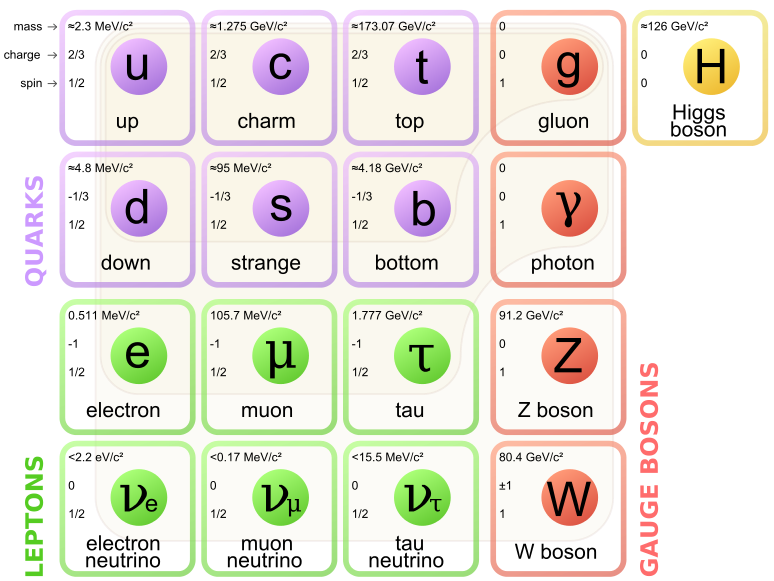
\includegraphics[width=0.9\textwidth]{figs/theory/iaGJO.png}
\caption{ The Standard Model Particle Content
 } \label{figure:theory_sm}
\end{figure}


\subsection{Electroweak Symmetry Breaking and the Higgs}

Despite the simple structure of theory, the discovery of massive fundamental
particles creates two sets of problems both related to $SU(2)_{L} \times U(1)$ symmetry. First, the force-carrying bosons must enter the theory
without mass or the symmetries will be explicitly broken in the Lagrangian. Second, adding
fermion masses to theory in an ad-hoc way allows the right-chiral and
left-chiral fermions to mix. Since they possesses different quantum numbers, as
different representations of the weak-isospin group, this too breaks gauge
invariance. 

To solve these problems, spontaneous electro-weak symmetry breaking (EWSB) is
introduced via the Brout-Englert-Higgs mechanism \cite{Higgs:1964pj, Higgs:1966ev,Englert:1964et}. A  massive scalar field
in an electro-weak doublet is added to the theory with 4 new
degrees of freedom and a potential which includes a 
quartic self-interaction term. Each fermion field interacts with the scalar field via
a different Yukawa coupling, which unites the left and right chiral fields
of a single particle type.  This field
explicitly preserves all of the symmetries, but the minimum of the potential does not
occur when the expectation of the field is zero. The field
eventually falls to a state, where it acquires a non-zero vacuum-expectation
value. A non-vanishing field must point in a
particular direction of weak-isospin space, breaking the symmetry.

The consequences of this spontaneous symmetry breaking are tremendous.
The universe is filled with a field that has a non-zero expectation value.
The theory can be expanded around this new value and 3 of the
degrees of freedom can be interpreted as the longitudinal polarizations of
the $W^+$, $W^-$, and $Z^0$, while the 4th remains a scalar field, called
the Higgs field with an associated particle called the Higgs particle or "Higgs".
The weak bosons acquire a mass via their longitudinal polarizations and the Yukawa
couplings of the scalar field to the fermions now behave like a mass term
at the this new minimum. 


\subsection{The Standard Model Parameters}


Confronting the SM with experiment requires the measurement of
17\footnote{There are additional parameters from neutrino mass terms and
mixing but it is unclear how to include these into the Standard Model,
since it does not predict right-chiral neutrinos} free parameters, which
are unconstrained from the theory. These free parameters include the fermion
masses from the Yukawa couplings, the force coupling constants, the angles and phase of the mixing between
quarks, and constants from the Higgs and electroweak sector\footnote{ The electroweak sector includes
parameters like mass of the $W^{\pm}$ and $Z^0$ bosons, the weak mixing
angle,${\mathrm sin^2}\theta_w$, the fermi constant $G_F$, and Higgs
Mass and vacuum expectation value. These parameters however are not
wholly independent. As discussed above, it is only necessary
theoretically to specify the two parameters relevant to the Higgs
potential and the two coupling associated with the gauge groups }.

%arXiv:1209.2716v2%
Experiments have provided a number of measurements of the
parameters of the SM\cite{lepew:2010vi}.  With the discovery of the Higgs boson and 
the measurement of the Higgs mass, all of the parameters
of the SM can be estimated and statistical procedures can assess
the relative agreement of overlapping measurements to test the self-consistency 
of the SM. The GFitter collaboration assembles
all relevant electroweak observable measurements into a statistical
model and then allows certain measurements to float within their
uncertainty to allow for a fit among multiple correlated measurements\cite{GFitter}. 
These correlations arise for two reasons. First, measurments are made that often
depend on multiple SM parameters. Second, radiative corrections often cause 
parameters to depend on each other. For instance, the Higgs mass is sensitive
to both the $W$ mass and top mass, through loop level corrections. 

Figure \ref{figure:theory_scans} shows the fitted constraints on 4 key SM
parameters ($M_H$, $M_W$, $M_t$, ${\mathrm sin^2}\theta_w$) with
actual measurements overlaid. The plots show both the removal
and inclusion in the fit of key measurements to assess their overall
impact. The addition to the fit of the measured
Higgs mass from the ATLAS and CMS collaborations creates a small
tension, as the other observables prefer the mass to be much
lower ($\sim$ 80 GeV). This tension in the combined
electroweak fit as a result is  not statistically
significant with a $p$-value of 0.07. The
SM seems to be self-consistent. 


\begin{figure}[!t]
\centering 
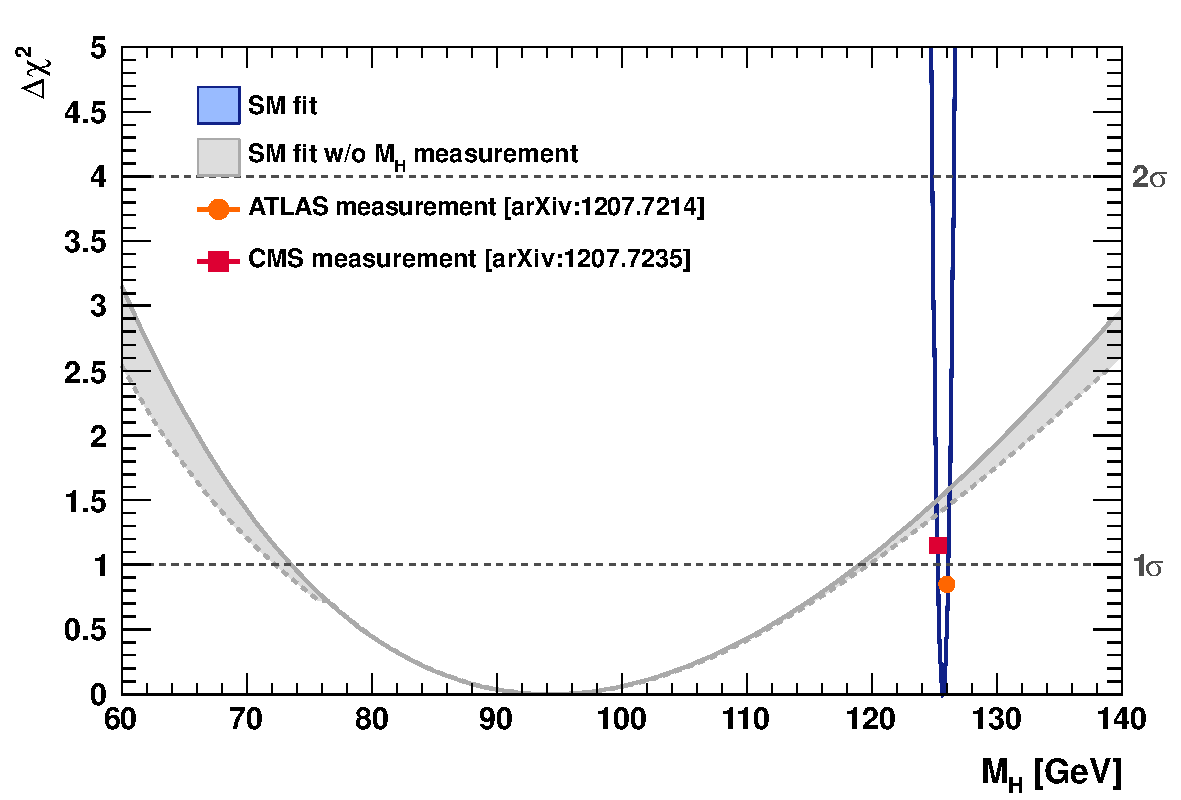
\includegraphics[width=0.45\textwidth]{figs/theory/HiggsScan.pdf}
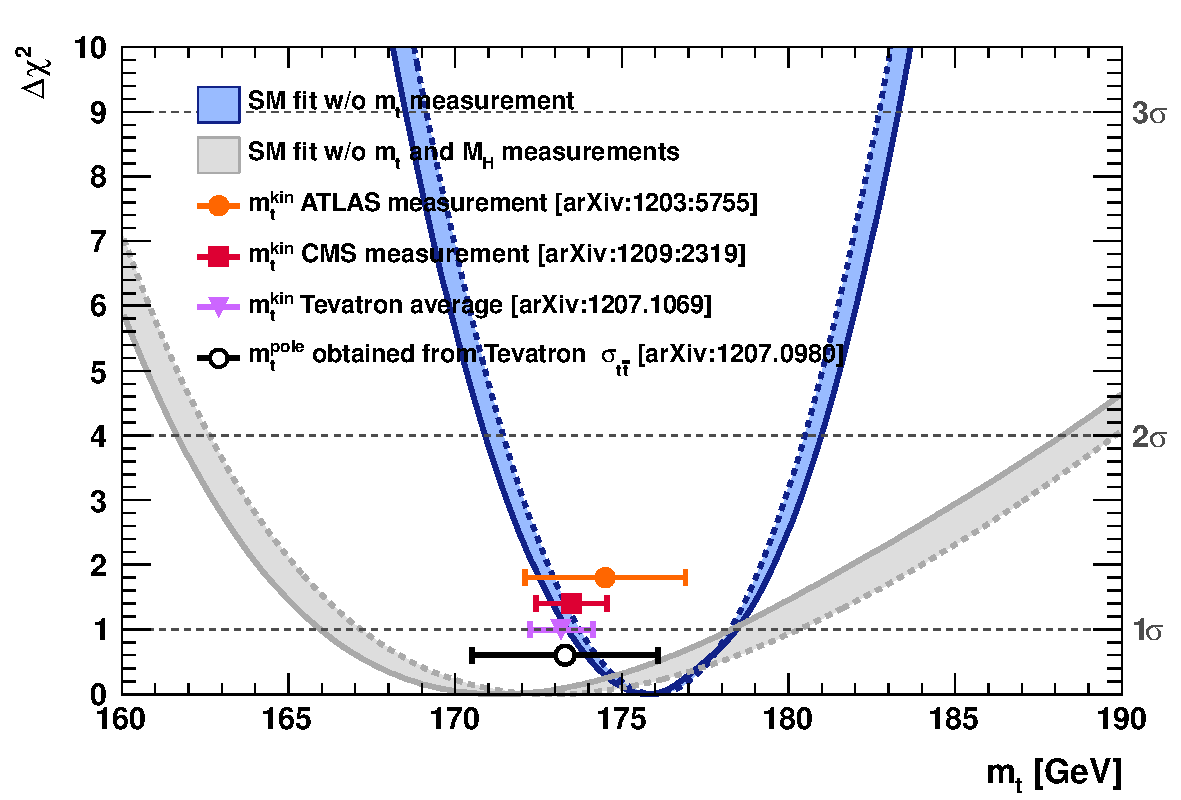
\includegraphics[width=0.45\textwidth]{figs/theory/TopScan.pdf}
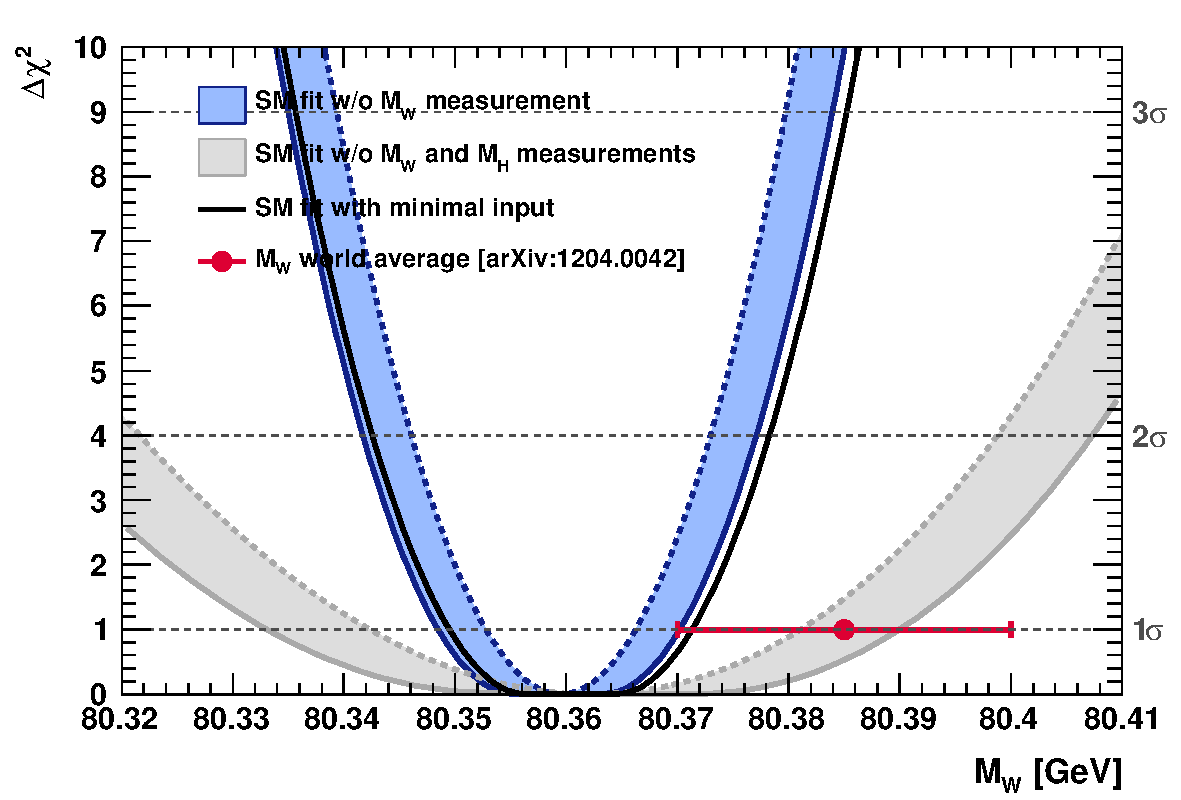
\includegraphics[width=0.45\textwidth]{figs/theory/WMassScan.pdf}
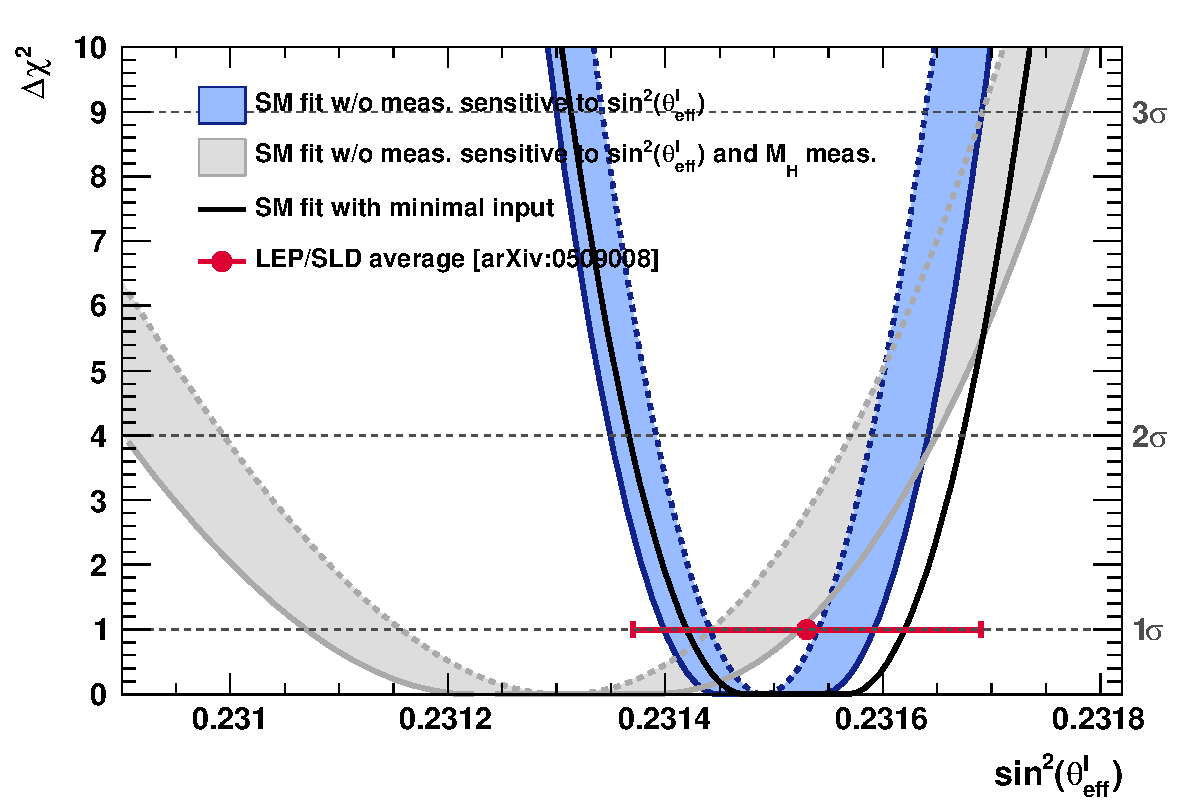
\includegraphics[width=0.45\textwidth]{figs/theory/Sin2ThetaScan.pdf}
\caption{
$\chi^2$ as a function of the Higgs mass (top left), the top quark mass (top
    right), the $W$ boson mass (bottom left) and the effective weak mixing
  angle (bottom right) for the combined SM fit from the GFitter group.  The
  data points placed along $\chi^2=1$ represent direct measurements of the
  respective observable and their $\pm 1\sigma$ uncertainties.  The grey (blue)
  bands show the results when excluding (including) the new $M_H$ measurements
  from (in) the fits. } \label{figure:theory_scans}
\end{figure}


\section{Collider Physics and the Higgs} 

To test the theory, physicists accelerate particles to extremely high energies and force
them to interact through collisions. Typically, the particles accelerated are
electrons or protons, since they are stable. Electron-positron collider
machines have a rich history of discovery and measurement in particle physics.
The advantage of electron accelerators is that the colliding element is itself
a fundamental particle. However, due to synchrotron radiation, the curvature of the
beam line becomes problematic for high energy beams.  On the other
hand, proton-proton and proton-anti-proton colliders can be accelerated in rings without large losses
due to synchrotron radiation, but the actual colliding objects at high
energies are the constituent quarks and gluons. This complicates analysis
because the initial state of the hard-scattering system is not known on a per-collision
basis and momentum of hard-scattering system is unknown along the beam direction.

For hadron colliders, physicists must rely on form-factor descriptions of the colliding hadrons
that describe the fraction of momentum carried by the
hadrons constituent 'partons'.  These are called parton-distribution
functions, seen in Figure \ref{figure:theory_pdf}, and are factorized
and integrated through the theoretical calculations of various collision processes \cite{1985.Collins.factorization-theorem}.

%http://arxiv.org/pdf/0901.0002v3.pdf
At the Large Hadron Collider or LHC, the collider used in this thesis, protons are collider.The types of initial hard-scattering statesat the LHC are quark-quark, quark-gluon, and gluon-gluon. Gluon collisions dominate overall,
  due to the large number of gluons inside the proton, though the relative importance of different initial states changes with the
  energy scale of the collision and the type of final state sought after.  

\begin{figure}[!t]
\centering 
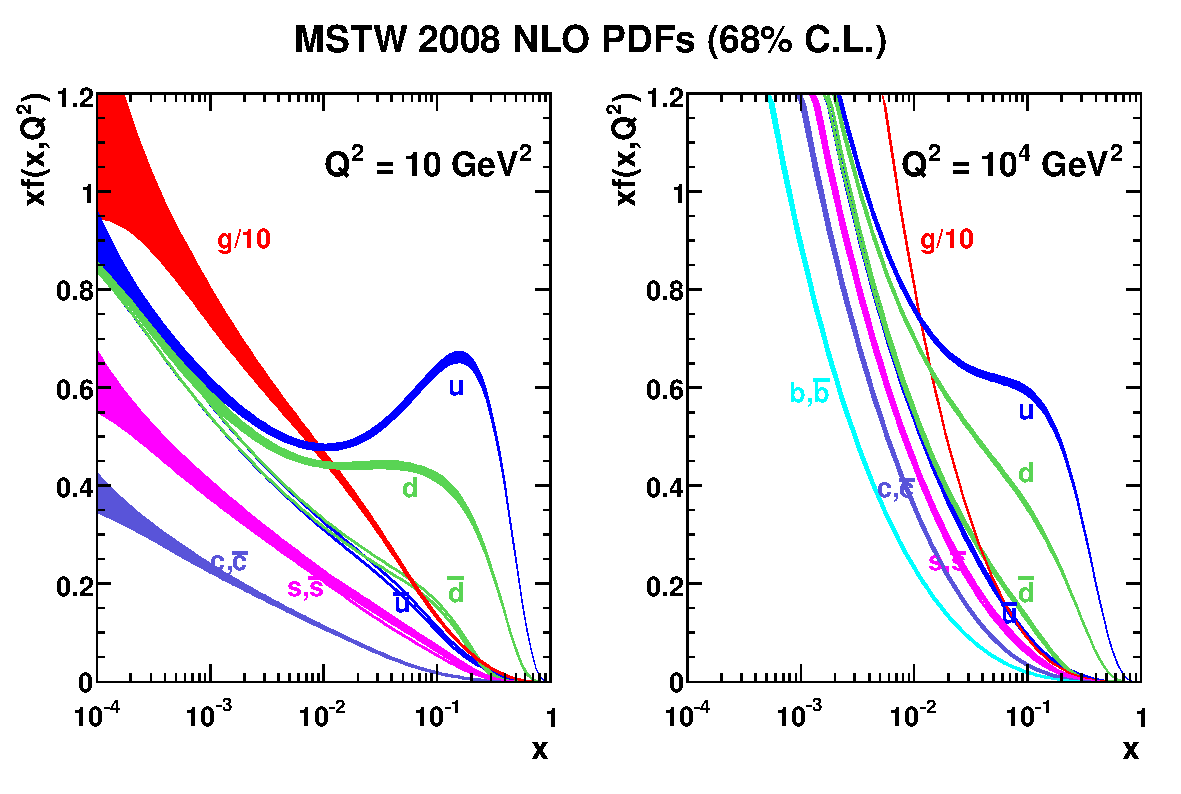
\includegraphics[width=0.8\textwidth]{figs/theory/mstw2008nlo68cl_allpdfs.pdf}
\caption {Proton Parton Distribution Functions (PDFs) form the MSTW Collaboration at $Q^2 = 10$ GeV$^2$ and $Q^2 = 10^4$ GeV$^2$}.
\label{figure:theory_pdf}
\end{figure}

%

%
A prime motivation for the construction of the Large Hadron Collider was the
discovery or exclusion of the Higgs boson\cite{lhcProposal}. LEP and the Tevatron excluded large
swaths of possible Higgs boson masses, especially below 114 GeV. The Higgs mass was also known to 
have a theoretically motivated upper bound. The unitarity of diagrams including the $WWWW$ vertex required the Higgs mass to
be below about 1 TeV.This LHC was thus designed to be able to eventually find or exclude 
a Higgs particle in this range \cite{lepew:2010vi}. 

Reaching this discovery oor exclusion required an enormous
dataset with collisions at high energies. Despite the fact that the Higgs couples to nearly
every particle, Higgs boson production at the LHC is a
low rate process. Because it couples to fermions proportional to mass and
because the colliding particles must be stable and therefore light, production
of the Higgs must occur through virtual states. 

\begin{figure}[!t]
\centering
\begin{tabular}{cc}
\subfloat[ggF]{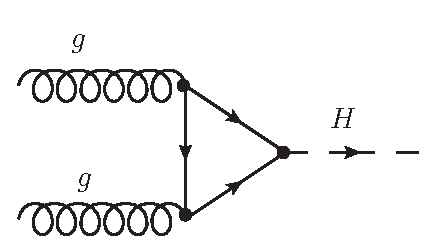
\includegraphics[width=0.35\textwidth]{figs/theory/ggF.pdf}} &
\subfloat[vbf]{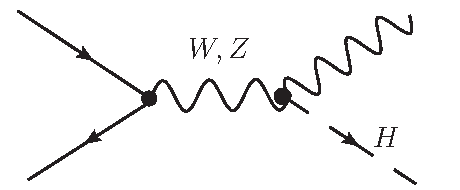
\includegraphics[width=0.35\textwidth]{figs/theory/vh.pdf}} \\
\subfloat[vh]{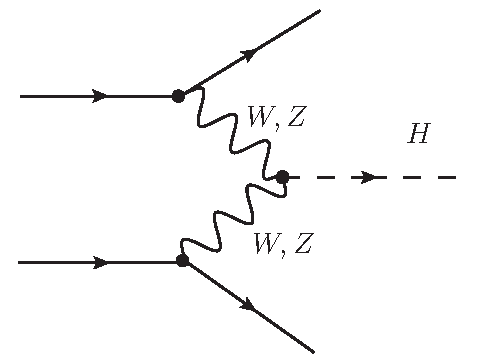
\includegraphics[width=0.35\textwidth]{figs/theory/vbf.pdf}} &
\subfloat[$t\bar{t}H$]{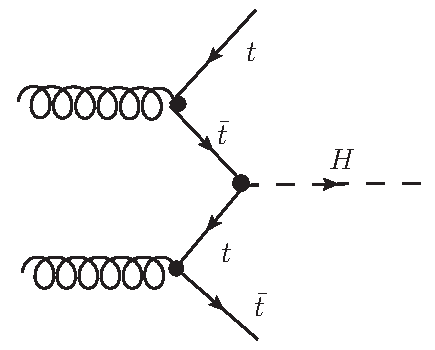
\includegraphics[width=0.35\textwidth]{figs/theory/tth.pdf}} \\
\end{tabular} 
\caption{Dominant Higgs production modes at the LHC}
\label{figure:theory_higgsdiagrams}
\end{figure}


The Higgs boson can be produced through collision at the LHC
via 4 mechanisms: gluon-fusion (ggF), vector-boson fusion (VBF), 
Higgsstrahlung (VH), and production in association with top quarks ($t\bar{t}H$). The diagrams
are shown in Figure \ref{figure:theory_higgsdiagrams} and the production
cross-sections as a function of Higgs mass for the 8 TeV LHC proton-proton
running are shown in Figure \ref{figure:theory_xsec} \cite{Dittmaier:2012vm}. The largest production
cross-section is via the gluon fusion channel at ~$20$ pb, which proceeds
through a fermion loop that is dominated by the top quark, because of its
large Yukawa coupling to the Higgs. Because the Higgs' couples to every massive
particle, it has a rich set of decays also seen in Figure
\ref{figure:theory_xsec}, especially for $m_H=125$.  Studies of Higgs
properties at hadron colliders offers many tests of the Standard Model
and ample room for searches for new physics. These
tests specifically can verify the link between Yukawa coupling and the
particles mass and further constrain details of EWSB by examining Higgs coupling
to the weak bosons. 

\begin{figure}[!t]
\centering 
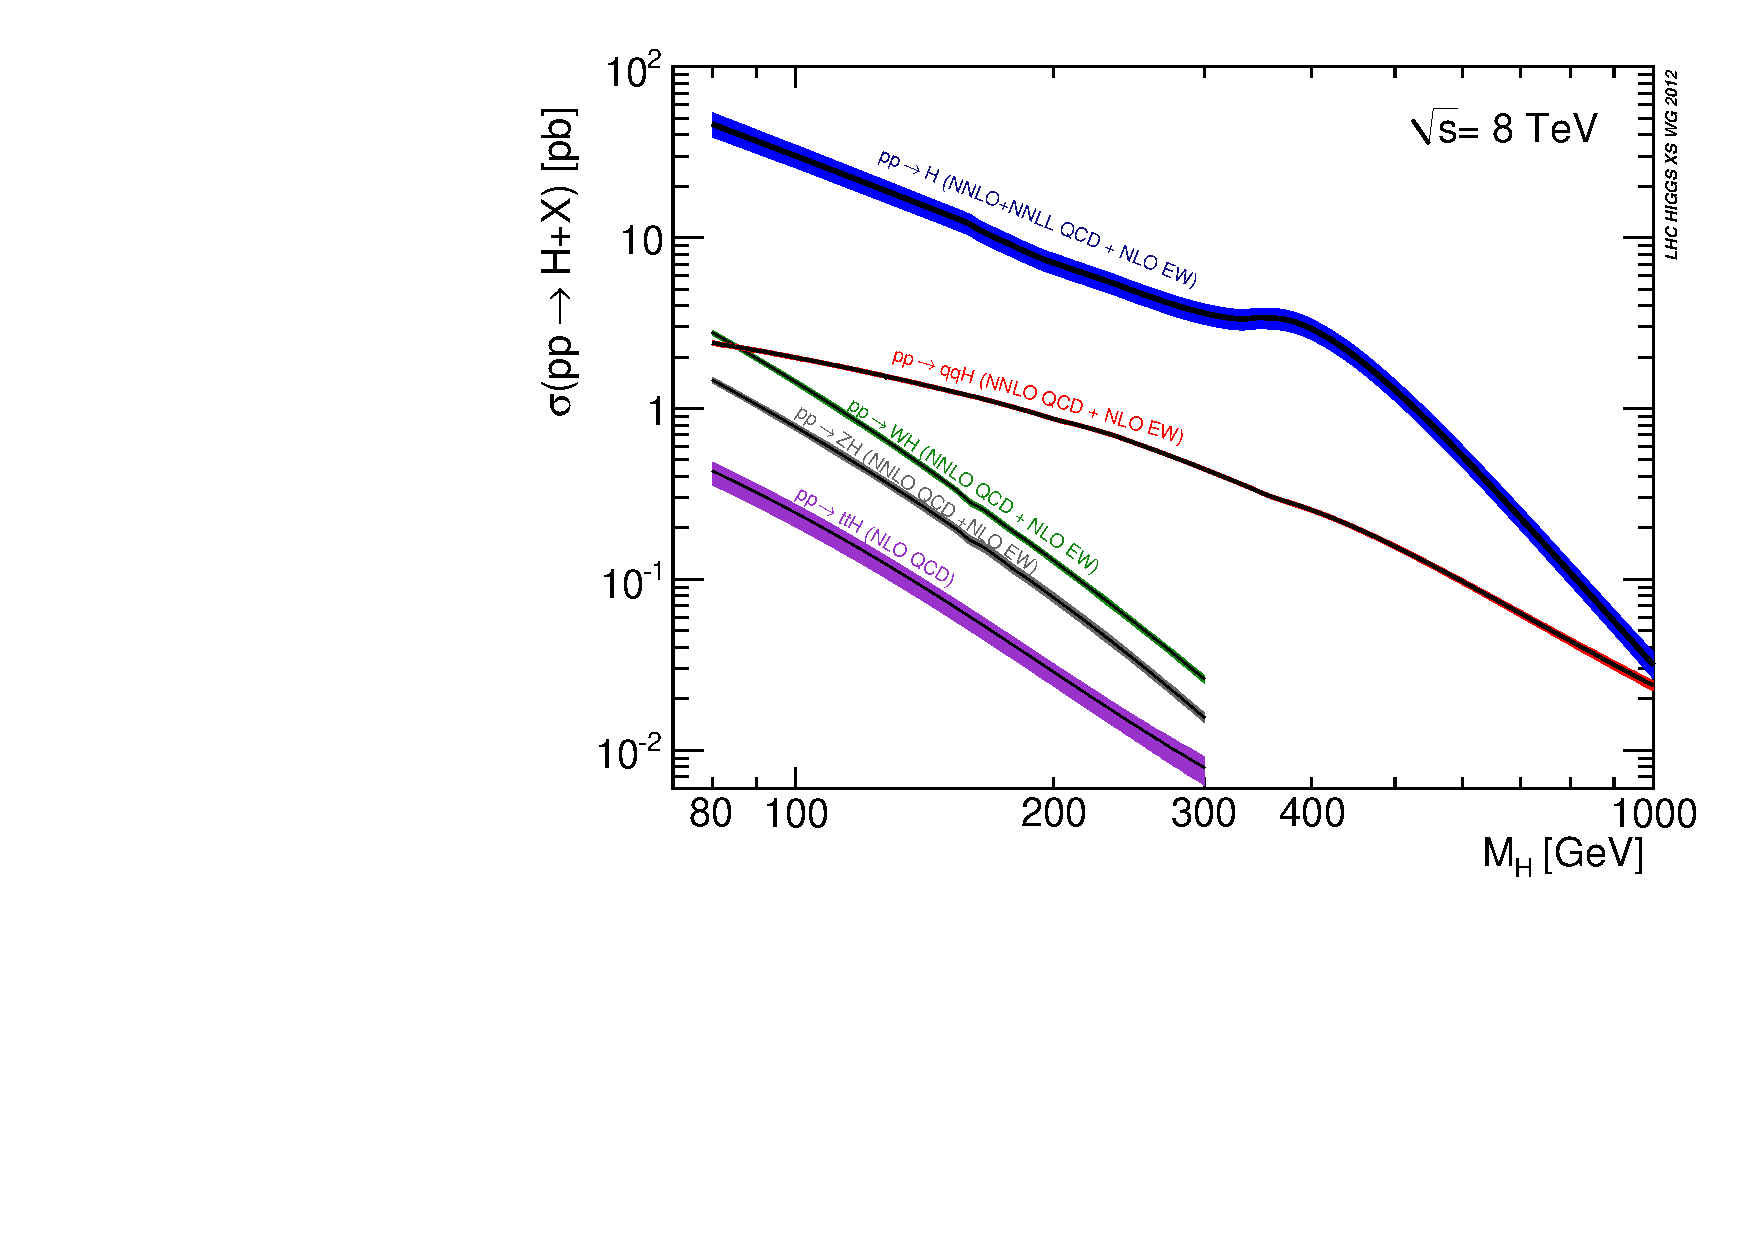
\includegraphics[width=0.52\textwidth]{figs/theory/Higgs_XS_8TeV_lx.pdf}
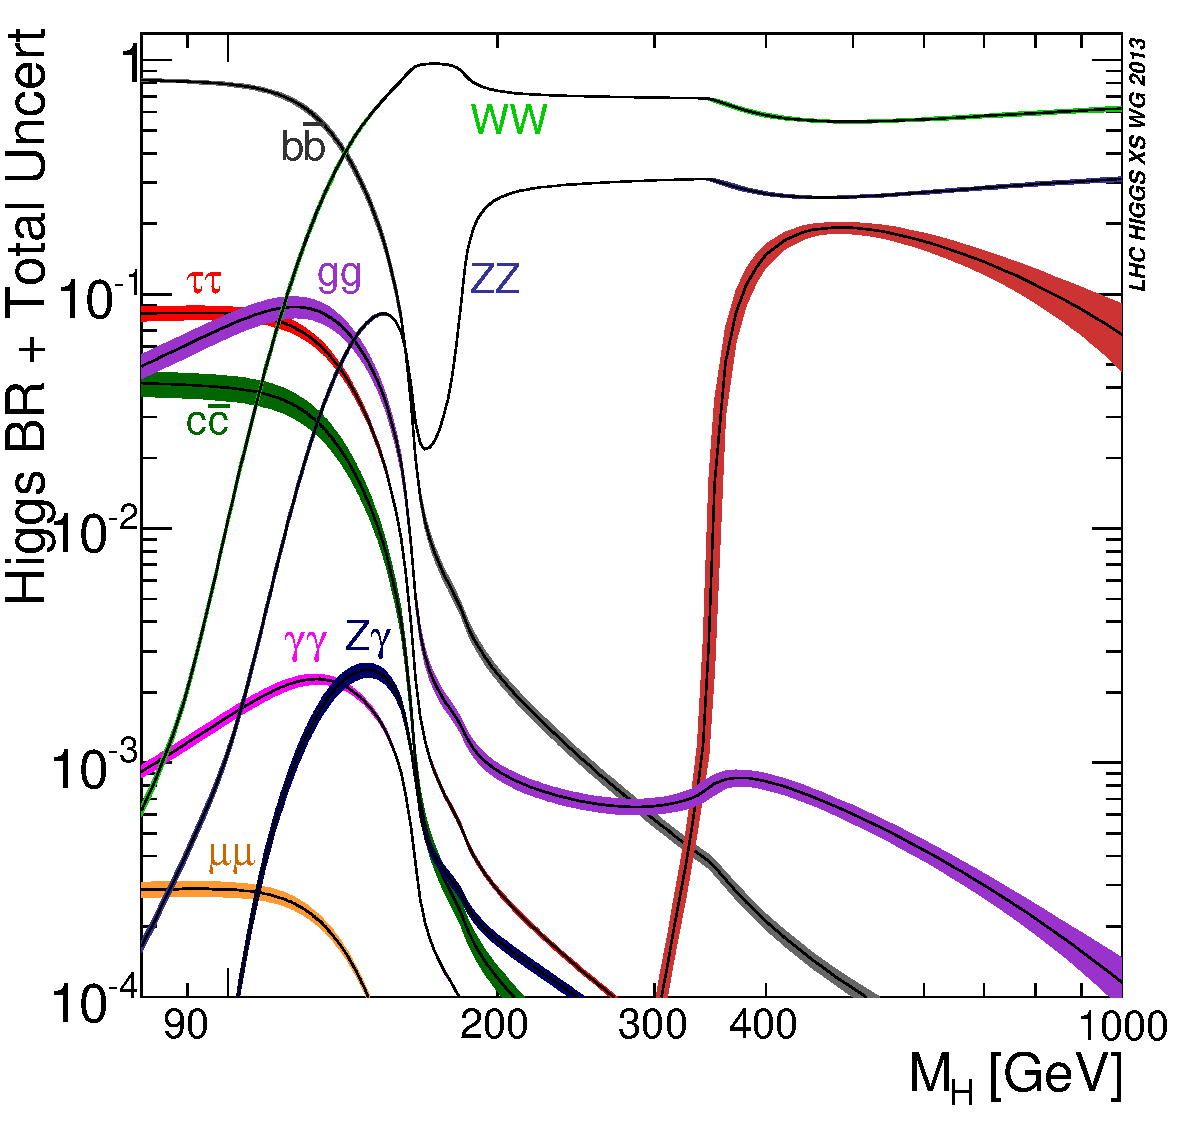
\includegraphics[width=0.42\textwidth]{figs/theory/Higgs_BR.pdf}
\caption {8 TeV LHC Higgs production cross-sections (left) and decay branching fractions }.
\label{figure:theory_xsec}
\end{figure}


\subsection{Higgs Discovery at the LHC}

In 2012 both ATLAS and CMS announced the discovery of a new boson consistent
with the Higgs by examining the results of Higgs searches in a number of decay
channels ($H\rightarrow W^+W^-$,$H\rightarrow Z^0Z^0$, and
    $H\rightarrow\gamma\gamma$) in the 2011 dataset at $\sqrt{s}=$7 TeV and
part of the 2012 dataset at $\sqrt{s}=$8 TeV. By 2013 and 2014, both
experiments have updated and/or finalized their results for the full 2011 and
2012 datasets \cite{ATLAS-CONF-2014-009,CMS-PAS-HIG-14-009}. I will focus on the ATLAS results in the following. 
ATLAS measured both the Higgs mass\cite{Aad:2014aba} and spin\cite{tagkey2013120}, as well as 
provided initial constraints of the Higgs couplings to different particles. 

Figure \ref{figure:theory_higgsdisc} show the results of the searches in all of the
measurement channels as well as constraints on the SM Higgs coupling parameters in 
an example fit, where the couplings to the top-quark, bottom-quark, W,Z, and $\tau$
are allowed to fluctuate independently. These rely on measurements binned in different
production and decay channels. They are dominated by higher statistics results in the 
gluon-fusion production modes, but measurements in the VH and VBF modes are close to 
SM sensitivity. 

The combined results show basic agreement with the SM with much room for improvement
with the addition of new production and decay modes and higher statistics. The 
coupling constraints are particularly strong for the W and Z, which are
the most sensitive decay channels, and top quark due to the dominance of the
top Yukawa in the ggF loop. 


\begin{figure}[!t]
\centering 
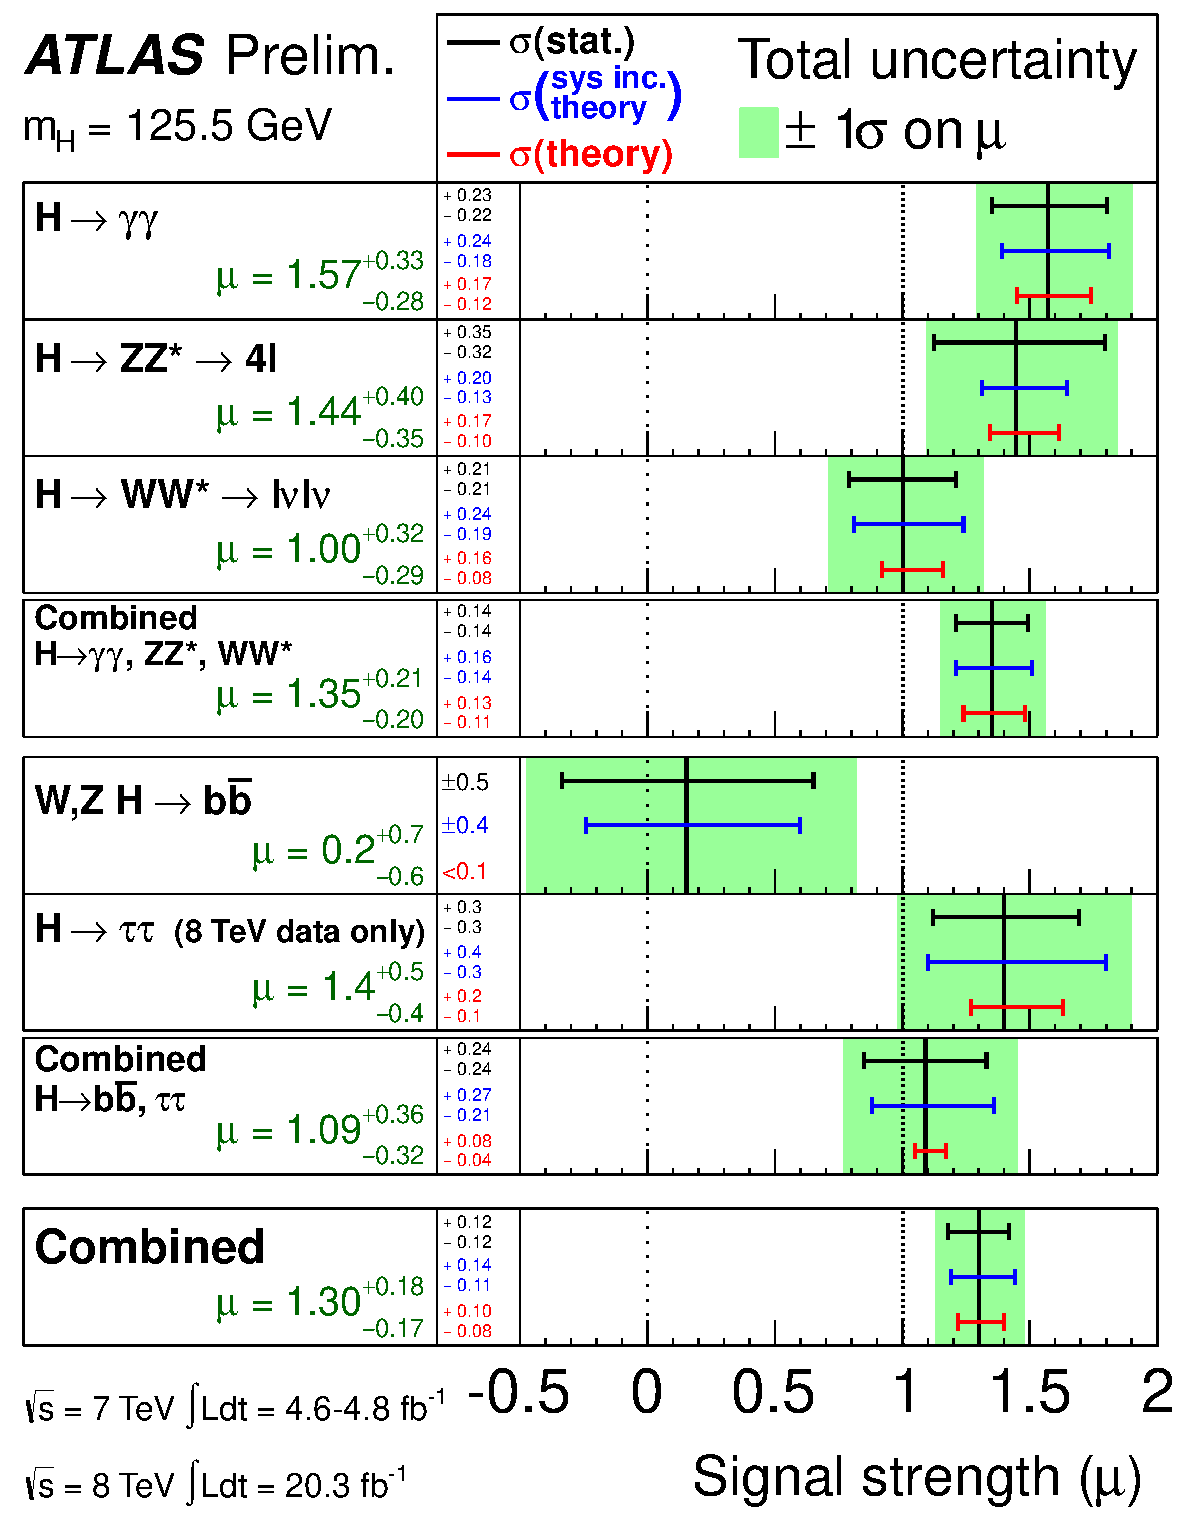
\includegraphics[width=0.45\textwidth]{figs/theory/atlas_higgs.pdf}
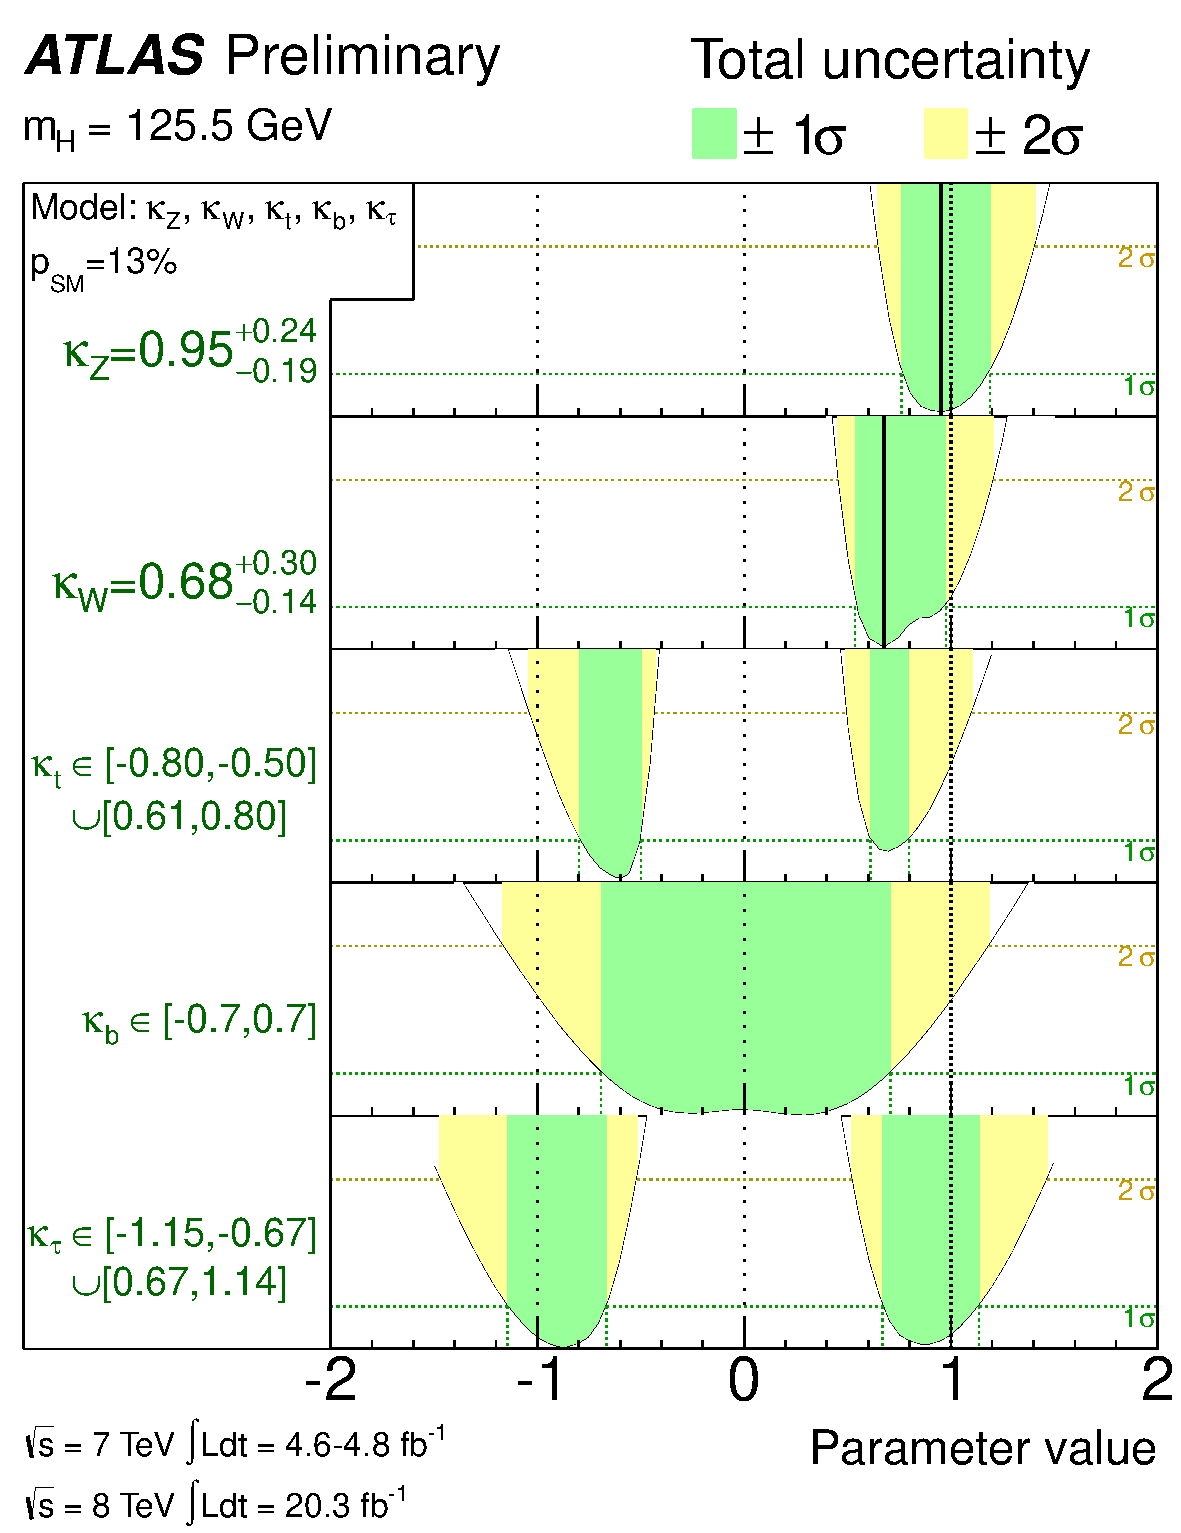
\includegraphics[width=0.45\textwidth]{figs/theory/atlas_coupling.pdf}
\caption {
  ATLAS Higgs combination results for all SM measurement channels as ratios of
  the measured to SM production cross-sections (left) and extracted Higgs
  coupling constraint scale-factors for a combined fit to the measurement
  channels, where the W,Z, top-quark, b-quark, and $\tau$ couplings are
  allowed to float. The p-value of this particular model is 0.13 and in agreement
  with SM expectations}

\label{figure:theory_higgsdisc}
\end{figure}


\subsection{The Importance $t\bar{t}H$ Production}

Notably absent thus far in the SM are searches for the Higgs in the $t\bar{t}H$
production channel, due to the low production rate and lack of statistics. Searches are underway and
initial results are close to SM sensitivity for ATLAS and CMS.

Measuring the $t\bar{t}H$ production rate is important, because
$t\bar{t}H$ production depends on the top Yukawa coupling at tree level. Comparing
the predicted Yukawa coupling from top mass measurements to the coupling from
the wholly independent Higgs production measurements is a very direct 
test of Higgs' invovlment in providing mass the fermions in the SM.

The top Yukawa coupling is already constrained from current measurements of the ggF production
process, since ggF loop is dominated by the top quark. However, new, colored particled could be
present in the loop. Comparison of the gluon-fusion and the $t\bar{t}H$
modes would allow for disentangling the effects of these possible new particles\cite{Dawson:2013bba}. 
The simplest of new phyiscs models, allowing for the modification
of the ggF loop, introduce a new generation of quarks. However, fourth
generation quarks, which obtain mass from a Higgs Yukawa coupling, are already
largely excluded due to their enormous effects on the Higgs production
cross-section\cite{Eberhardt:2012gv}. Other exotic scenarios allow for new colored particles, 
which are not entirely constrained by present measurements\cite{Carena:2013iba,ArkaniHamed:2012kq,Carmi:2012yp}.
These include, for instance, supersymmetric models involving the stop quark.  

With the level of statistics available in Run I dataset, very strict constraints on the top 
Yukawa coupling are simply not possible and the measurment presented in this 
thesis is a first stemp. Future, high-statistics datasets will have the ability to provide 
better measurments and \tth production will become very important.
Despite similar uncertainties on the overall production cross-sections for $t\bar{t}H$ and the ggF,
\tth has the advantage that most of these uncertainties would cancel for $t\bar{t}H$ if normalized to the topologically similar $t\bar{t}Z$.  Finally, the uniqueness of the experimental signature means that
searches for $t\bar{t}$ signatures can be performed for a variety of Higgs decays ($\gamma\gamma$, $b\bar{b}$,
$WW$,$ZZ$, and $\tau\bar{\tau}$ with roughly similar degrees of sensitivity (within a factor of 10)\cite{Dawson:2013bba}. 


It is important to note the importance of the top Yukawa coupling
due to its enormous size compared to other couplings. For instance, the top Yukawa is 350000x as large as the electron
Yukawa coupling. The top Yukawa coupling,
along with the Higgs mass, is one of the most important pieces of the renormalization group equations (RGE)
responsible for the running of the parameter that determines the Higgs self-coupling $\lambda$. 
If this parameter runs negative, then the potential responsible for the entire mechanism 
of EWSB no longer has a minimum and becomes unbounded, resulting in instability in the universe \cite{Degrassi:2012ry}.
Metastability occurs when the shape of the potential allows for a false local minimum.
Figure \ref{figure:theory_stability} shows the running of this parameter, the regions
for which the universe is stable, unstable and metastable. Current
measurements suggest that universe lies in a metastable island\footnote{The
RGE assumed that there is no new physics at all energy scales}. This is a sort of fanciful
aside, intended only to highlight the importance of the top Yukawa coupling and to suggest that
new discoveries in the top-Higgs sector have far reaching consequences. 


\begin{figure}[!t]
\centering 
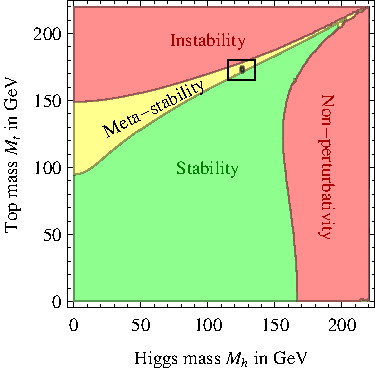
\includegraphics[width=0.45\textwidth]{figs/theory/SMstability.pdf}
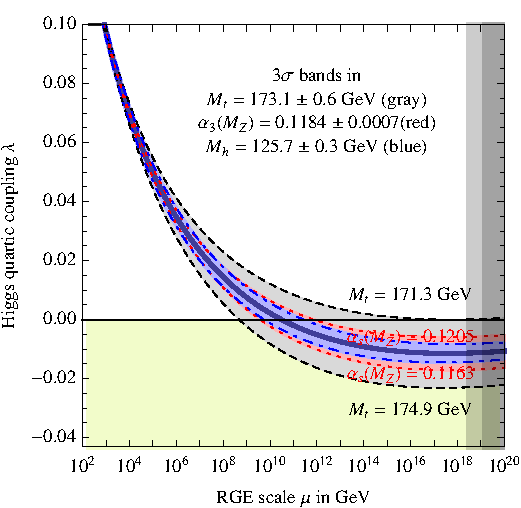
\includegraphics[width=0.45\textwidth]{figs/theory/runLambda.pdf}
\caption {
  RGE for the running of the SM parameter, $\lambda$ for the Higgs self-coupling term 
  with present values and uncertainty bands for $M_H$ and $M_t$ (left). The two-dimensional
  plot colored (right) shows regions for which the SM is stable, unstable, and metastable
  based on this RGE}

\label{figure:theory_stability}

\end{figure}


\section{Conclusion}

The Standard Model, despite its success in providing a unified description of fundamental
particles and interactions into single theory, has its flaws. These have been discussed in 
depth elsewhere, but include issues like the description of massive neutrinos, the failure
to include gravity, and the unnaturalness of large quantum corrections to Higgs parameters.
For these reasons, it seems the SM might be a lower energy approximation to a more fundamental
theory. The discovery of the Higgs boson at the LHC provided a stunning verification of one
of the fundamental aspects of the theory but at the same time offers new area to search for
glimpses of something grander. The production of samples of Higgs bosons
allows for a rich array of new tests of the Standard Model, which is now finally over-constrained by experiment. 
Searches for the $t\bar{t}H$ production, one category of which is the topic
of this thesis, provide tree-level access to a central parameter of the theory, the top Yukawa coupling,
as well as access a variety of Higgs decays, which will eventually provide a rigorous new 
test of the SM. 



%% \chapter[htoc-titlei][hhead-titlei]{htitlei}
%% -----------------------------------------------------------------------------
\chapter[The Large Hadron Collider][The Large Hadron Collider]{The Large Hadron Collider}
<<<<<<< HEAD
%test
Production of a sufficient number of high energy collisions to adequately explore
particle physics at the electro-weak scale required the development of one
of the most complex machines ever built, the Large Hadron Collider or LHC. This chapter
provides a very brief overview of the machine with particular focus on the 2012
dataset of proton-proton collisions it enabled. 
The technology involved in the development of the LHC and very breifly
touched upon in this chapter is an enormous achievement
it its own right and is documented in detail here \cite{1748-0221-3-08-S08001,Pettersson:291782,Linnecar:1176380}. 


\section{The Large Hadron Collider}

The LHC is the world's highest energy particle accellerator 
=======
\section{The Large Hadron Collider}

The Large Hadron Collider(LHC) is the world's highest energy particle accellerator 
>>>>>>> FETCH_HEAD
and is located 100m underneath the Franco-Swiss border at the European Organization
for Nuclear Research (CERN) in a 26.7 km tunnel. 

The LHC is a ciruclar 
machine capable of accelerating beams of protons and colliding them at center of mass 
energies up to $\sqrt{s} = 14 TeV$ at 4 collision sites around the ring, where 4 experiments
<<<<<<< HEAD
are housed (ATLAS\cite{ATLAS_detector}, CMS\cite{748-0221-3-08-S08004}, LHCb\cite{1748-0221-3-08-S08005}, and ALICE\cite{1748-0221-3-08-S08002)}. Figure \ref{figure:lhc_lhc} is a diagram
of the layout of the LHC and its experiments\cite{Team:40525}. The LHC also operates in a modes with beams of 
heavy ions. The LHC is composed of thousands of super-conducting Niobium-Titantium 
magnets, cooled to 2.7$^\circ$ C with liquid Helium, which steer and focus the 
particle beams, and a superconducting resonant-frequency (RF) cavity,which boosts the beam
to higher energies. 

% magnets
\begin{figure}[!t]
\centering 
\includegraphics[width=0.35\textwidth]{figs/lhc.pdf}
\caption{ Diagram of the Large Hadron collider and location of the 4 main experiments (ATLAS, CMS, LHCb, and ALICE). Around
  the ring. The diagram also shows the location of the SPS, the final booster ring the accelerator complex that accelerates
    the protons to 450 GeV before injection into the LHC. 
}
\label{figure:lhc_lhc}
\end{figure}



\subsection{The Accelerator Complex}

The accelerator complex is a progressive series of machines that progressively boost
the particle beams to their final beam energy and intenstiy.
=======
are housed (ATLAS, CMS, LHCb, and ALICE). The LHC also operates in a modes with beams of 
heavy ions. The LHC is composed of thousands of super-conducting Niobium-Titantium 
magnets, cooled to 2.7$^\circ$ degrees
% magnets


The technology involved in the development of the LHC is an enormous achievement
it its own right and is documented in detail here. 

\subsection{The Accelerator Complex}

The accelerator complex is a progressive series of machineswith the LHC as the final stage.
>>>>>>> FETCH_HEAD
Protons are obtained from hydrogen atoms and are accelerated to 50 MeV using the
Linac2, before being injected into the Proton-Synchrotron Booster (PSB). In
the PSB the protons are accelerated to energies of 1.4 GeV for injection
in to the Proton-Synchrotron (PS). The PS accelerates the protons to 25 GeV
and dumps bunches into the Super Proton Synchrotron (SPS), where they 
are accelerated to 450 GeV and finally dumped into the LHC. 

\subsection{Beam Parameters and Collisions} 

<<<<<<< HEAD
For the physics studied at the ATLAS experiment, the two most important parameters of
the collisions provided by the LHC are the center of mass energy and instantaneous luminosity.
High center of mass energies are necessary for the production
of new high mass particles, and because the consitutents of the actual collisions
are the partons of the proton, the CME of the collisions must in general
be much higher than the mass of the particles needed to be produced. The

\begin{figure}[!t]
\centering 
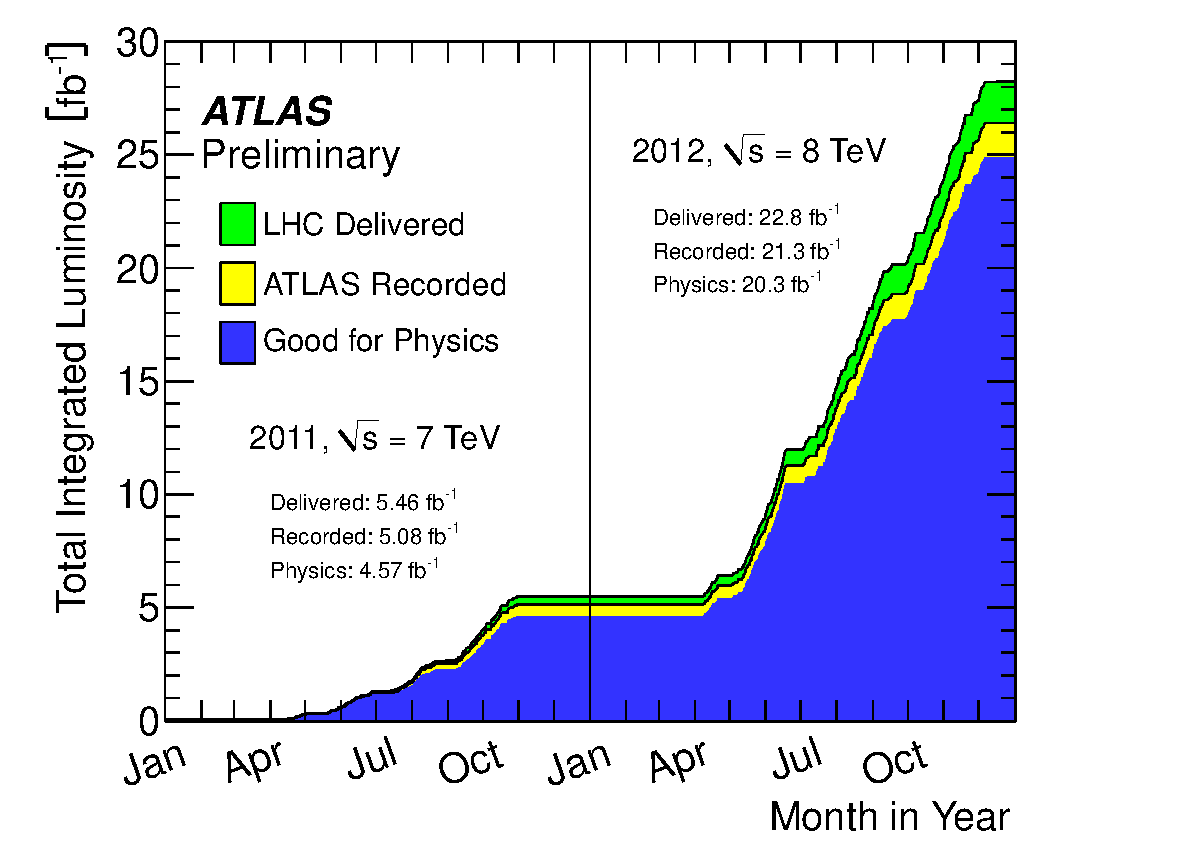
\includegraphics[width=0.35\textwidth]{figs/intlumivstime2011-2012DQ.pdf}
\caption{ Plot showing the accumulation of the integrated lumonisity delivered to the ATLAS experiment over 2011 and 2012. The rough size of the usable, physics ready dataset for 2012 is 20 $fb^-1$ and is the dataset used for the following analysis. 
}
\label{figure:lhc_lumi}
\end{figure}
The instantaneous luminosty of the collisions, \mathscr{L}, is a measure of the
collision rate. The integrated luminosity over time is a measure of the size
of the dataset and when multiplied by the cross-section of a particular process
gives the total number of expected events produced for that process.
Instantaneous luminosity depends on the number of colliding bunches of protons,
the intensity of those bunches, the revolution
frequency, and the nomralized transvserse spread of the beam in momentum and position
phase space, called the emmitance, and the transverse beam size. The LHC has the
option for colliding beams with 2808 bunches of protons, each with around $10^11$ protons,
at a rate of one bunch collision every 25 ns, or 40 MHz. These correspond
to a design luminosity of around $10^34$ cm$^{2}$ s$^-1$ or 10 nb$^-1$ s$^-1$
  
\section{The 2012 Dataset} 

The LHC successfully produced datasets for physics studies in 2010, 2011 and 2012. The 2012 
proton-proton dataset was delivered with collisions with a CME of 8 TeV with bunch collisions
every 50 ns and reached a total integrated luminosity of around ~20 fb$^-1$ \cite{Aad:2013ucp}.
Figure\ref{figure:lhc_lumi} shows the accumulation of this dataset over time. 
The full LHC design energy was never reached due to worries about faulty dipole
connections invovled in the unexpected quenching of the magnets in 2008. Despite doubling
the bunch spacing (thereby halving the bunch collision frequency), the lumonisty neared
the design lumonisty due to unexpected improvements in the transverse beam profile\cite{Carli:1424362}. This increased
the amout of pile-up, or number of collisions per bunch crossing and in general collision
events were busier due to these multiple interactions\cite{}. Figure \ref{figure:lhc_pileup} shows
the average number of interaction per bunch crossing for the 2011 and 2012 datasets. The 2012
dataset shows an average of 20-25 interactions. 

\begin{figure}[!t]
\centering 
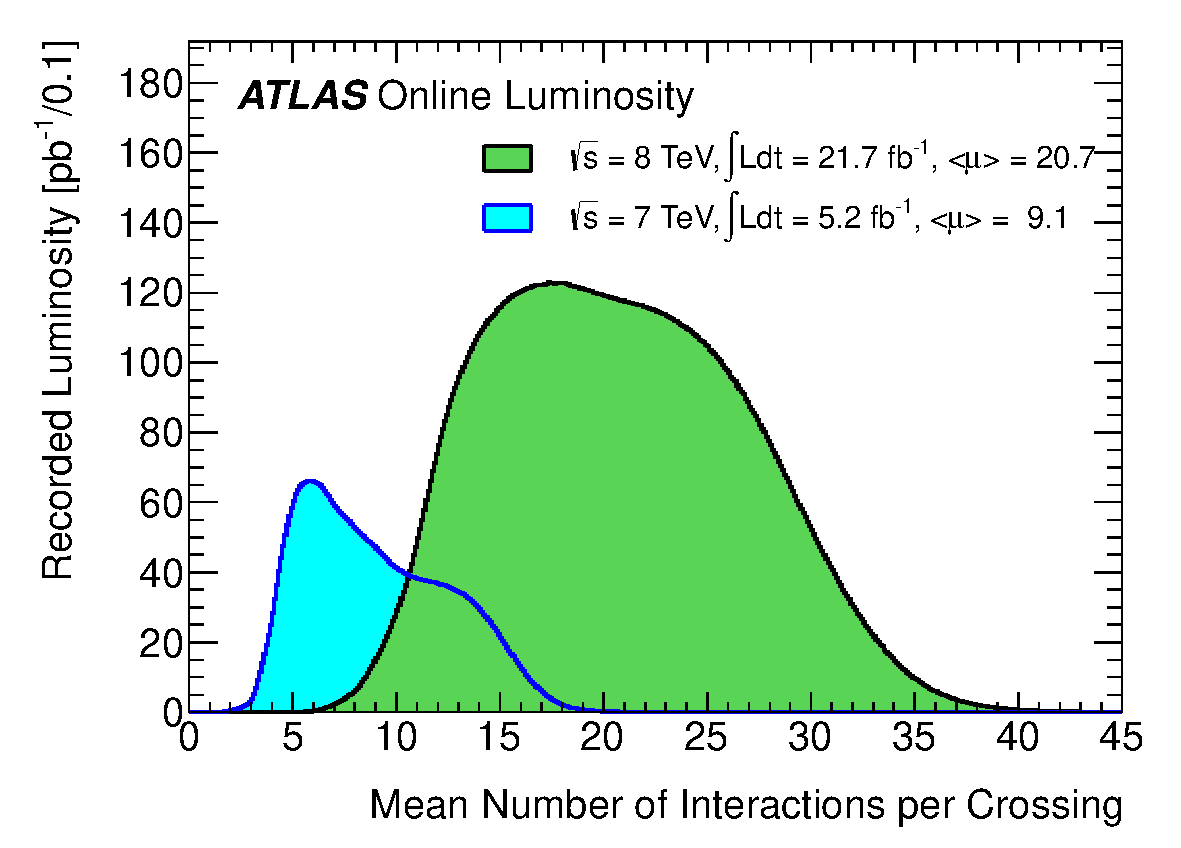
\includegraphics[width=0.35\textwidth]{figs/mu_2011_2012-dec.pdf}
\caption{ The average number of interactions per bunch-crossing for the 2012 and 2011 LHC proton-proton dataset. Most of these interactions are unintersting but leave energetic signatures in particle detectors called pile-up which interfere with measurements}\label{figure:lhc_pileup}

=======



\section{The 2012 Dataset} 
>>>>>>> FETCH_HEAD

\chapter[Electrons][Electrons]{Electrons}
\label{chapter:electron} 

High energy electron signatures are important elements of seaches and measurements at hadron colliders, because they signal the presence of important electo-weak processes in the event. Requiring well-identified electrons in collision events quickly suppresses the overwhelming rate of strong-force mediated scattering and allows for the collection of a manageably-sized dataset with intersting physics for study. For this reason, electron signatures form one of the two pillars of the HLT trigger at ATLAS, as discussed in Chapter~\ref{chatper:lhc} and rigorous electron identification is an important peice of many ATLAS analyses. This section summarizes the development of ATLAS electron identification for the high luminosity 2011 and 2012 datasets and discusses the techqniues invovled in measuring the electron identification efficiency. 

\section{Identification of Electrons at ATLAS}

%picutres and example figures

Electron reconstruction is discussed briefly in Chapter~\ref{chatper:lhc} and, in depth here~\cite{}. The result of electron reconstruction is called an electron candidate, which is comprised of a narrow calorimeter energy cluster with $|\eta| < 2.47$ and inner detector track that matches loosely in $\eta$ and $\phi$. If the electron has $|\eta| < 2.01$, the the inner detector track is fiducial to the TRT has has the possibility of having high-threshold hits, indicative of transition radiation (TR). Electron cluster recontruction is extremely efficient. The track-matching requirement is less efficient, because the presence of hard bremsstrahlung may in certain cases cause the electron cluster and emitted photon cluster to have a wide separation in the calorimeter\cite{}. 

Objects that are not isolated electrons are often reconstructed as electrons, as the reconstruction requirements are quite loose. Objects that often `fake' isolated electrons are light quark and gluon jets, heavy flavor jets that include real decays to electrons and converted photons. Light quark and gluon jets fragment into a number of collimated hadronic particles. In rare cases, the jet may fragment most of its energy into a single charged pion, which showers early in the EM calorimeter. In other rare cases, the jet may fragment mostly into a neutral pion, which subsequently decays into a pair of photons. If one of these photons converts, a track will point to the EM energy cluster. These cases would result in a reconstructed electron candidate. Although the probability for this to happen is small, the enormous jet production rate means that it is a significant background. In general, light quark and gluon jet `fakes' have larger transverse shower profiles and more energy leakage into the hadronic calorimeter. For the neutral pion case, there are generally two separated showers for lower energy decays. For both cases, there are often other particle signatures nearby.  
On the other hand, heavy-flavor jet decays and photon conversions contain real electrons. However, heavy flavor decays also involve the production of additional hadronic particles within the jet and both photon conversion and heavy flavor decays involved secondary vertices displaced from the primary interaction point. 

In order to distinguish these fake signatures from real isolated electrons, electron identification algorithms use a number of reconstructed variables describing the electron shower in the detector and the electron track. The details of the calculated variables can be found here~\cite{}. In general, the calorimeter variables take advantage of the narrowness of isolated electron shower in the transverse plane and lack of energy deposition in the hadronic calorimeter. The transverse variables include measurements of the shower width in both layer 2 and the strips, where more refined measurements are possible. In fact, the strips were designed to separate single photon and eletron showers from multiple showers from neutral pion decays, shown in Figure \ref{}. The shower width variables are generally measured mostly in $\eta$ as bremstrahlung tends to smear the electron energy in $\phi$. Electron tracks are required to have an adequate number of hits in the Pixel Detector, SCT and TRT. These hit requirements, especially the b-layer requirment suppress electron conversions which occur in the detector material. Track-cluster matching and geometric impact parameter variables require ID tracks to match the calorimeter energy well and to arise from the primary interaction point, respectively. Electrons with tracks explictly associated with a conversion vertex may be rejected. Finally, the high threshold fraction of hits on the track, made by transition radiation is an uncorrelated discrimator of pion and electron tracks.


Electron identification algorithms make selections in 9 bins of $|\eta|$, [0.10, 0.60, 0.80, 1.10. 1.37, 1.52, 1.81, 2.01, 2.37, 2.47] and bins of \pt, [7, 10, 15, 20, 30, 40, 50, 60, 70, 80$+$]. The $|\eta|$ binning changes with the calorimeter geometry, which in turn affect the shower shape distributions. The shape of most of the identification variable distributions, tracking and calorimeter, are \pt\ dependent.  


\begin{figure}

\end{figure}

\subsection{Pile-up and Electron identifiation}

\subsection{2011 Menu}

Electron identification in 2011 was accomplished through rectangular cuts on the identification variables at 3 operating points: Loose, Medium and Tight. The medium operating point was used online as the primary electron trigger. At the bbeginning of the 2011 run, the 3 operating points possessed the same cuts, but tighter operating points had cuts on more variables. The Loose operating point only cut on shower shape variables in layer 2 and hadronic leakage, the medium operating point added cuts on shower width variables in the strips, and tight added TR cuts, strict-track cluster matching, conversion rejection and a b-layer requirement. This menu, called the `IsEM' menu, was the first fully data-optmized cut menu for electrons. 

The demands of increasing luminostiy demanded a tightening of the medium operating point midway through the data-taking, in order to maintain a EF trigger rate of around 20-25 Hz on the primary electron trigger. To accomplish this, variables cut on at the tight operating point were added to the medium operating point, and the entire set of cuts was optimized to provide the targeted fake rejection and reduction in the rates at the highest possible efficiency. The same procedure was applied to the loose operating point, where the target was to provide efficiencies of 95\% and the highest possible fake rejection. The re-inventing of the menu in this way allowed for not only better performance, due to the inclusion of more variable, but a more stable tightening of the backgrounds from loose to medium to tight, where the same backgrounds types were targeted at each level. The new menu was called the `IsEM$++$' menu and the operating points were renamed `Loose$++$', `Medium$++$' and `Tight$++$'. Figure \ref{} shows the comparison of the operating points for the new menu and old menu.

\subsection{2012 Menu and Pile-up}

Improvements in the running conditions for 2012, in particular narrowing the transverse beam emittance and size, resulted in large increase in number of proton-proton interactions during every 50 ns bunch crossing. In 2011 the average number of reconstructed primary vertices in each event, an indicator of the number of interaction per bunch crossing, was around 7, while in 2012 the average grew to 25. Some events during 2012 running had 40 reconstructed primary vertices.

The increase in energy in the calorimeters from these additional collisions, called pile-up, caused a worsening of the resolution of electron identification variables, particularly the shower shapes and hadronic leakage.The presumed cause was the increase in the number of showers of low energy hadronic particles nearby electrons.  Figure~\ref{} shows an example distribution, the hadronic leakage under different pile-up conditions. The distributions shows a clear widening which results in a loss of efficiency. 

In order to combat this loss, the `IsEM$++$' menu was once again optimized to have a flatter efficiency profile as a function of the amount of pile-up in the event with similar perfromance to the 2011 menu. The strategy for this menu was to loosen selections on variables sensitive to pile-up energy. It was expected and confirmed that relying more on the strip variables for the shower shape selection and the energy in layer 3 of the EM calorimeter for the hadronic leakage, would use a smaller volume of the calorimeter and thus be less sensitive to additional energy in the neighborhood of the electron. The strategy is outlined pictorally in Figure~\ref{}.  

The efficiency of the 2011 operating points compared to the 2012 operating points is shown in Figure~\ref{}, demonstrating a clear improvement in effiency of the selections for higher pile-up conditions. Finally, the 2012 primary electron trigger to include highly efficient tracking isolation criteria in order to 

\subsection{Electron Likelihood}

A natural step forward for the electron identification is the use of multi-variate algorithms. Multi-variate identification algorithms use many identification variables at once in a multi-dimensional space and judge where signals and backgrounds are found in that space to make decisions

For the case of electron identification, it was found that using a likelihood function, trained with electron identification variables, provided clear perfmance gains with respect to rectangular cuts, while also providing stable and easily understandable results. The likelihood scores each electron based on how signal-like or background  it is for each individual indentification variable and then multiplies these identification variables together into a final score. Figure~\ref{} shows 

XXX equations?


There are many advantageous to a likelihood based approach. First, variables that show signficant shape differences between real and fake electrons but do not have a clear cut point can still be used in a likelihood. Second, the likeihood score takes into account the entire shape of the distribution and not simply an efficiency and fake rejection at a single cut point. Finally, the final cut on the likelihood output score.

The likelihood menu for ATLAS was developed at the end of the 2012 Run to be used on advanced 2012 analyses. The menu uses similar variables to the cut-based menus but adds a few additional variables, including a measurement of the amount of energy the electron track lost as it traversed the ID. The likeihood menu makes cuts on the likelihood output score at 4 different operating points with the same binning as the cut menu but tunes the cuts based on the amount of pile-up in the event. The likelihood menu greatly outperforms the rejection of the `IsEM$++$' menu for similar efficiencies. Figure XXX shows. The likelihood menu, specificaly the \textsc{verytight} operating point, is used in the \tth\ analysis.  

\section{Measurement of Electron Identification Efficiency at ATLAS}

Precise measurements of the electron identification efficiency are important pieces of many ATLAS analyses, including the \tth\ multi-leptons analysis. For analyses with low \pt\ leptons, systematic uncertainties on the electron identification efficency can be some of the largest sysetmatic effects. The methods used to measure the electron identification efficiency are described in depth here \cite{}. 

Electron identifications efficiencies are measured using a method called tag-and-probe for $J/\Psi$ and $Z$ boson decays to electrons. One object from the decay is tagged, while the other electrons is left unidentified. Reasonable confidence that the second object, thought not identified, is an electron based on the kinematic properties of the event, specifically the di-electron invariant mass is near the $Z$ of $J/\Psi$ pole. The tag-and-probe method leaves a sample of unidentified and unbiased probes, where the efficiency can be measured.

As opposed to muons, contamination from fake electron make the tag-and-probe method difficult. This is especially true for electrons in with \pt\ of 10-20 GeV. The energy scale of $Z$ and $J/\Psi$ decays disfavor electrons of this momentum, but low energy electrons are important in a number of Higgs searches. Backgrounds from fake electrons are subtracted using fits to the $Z$ and $J/\Psi$ invariant mass distributions. For $Z$ electrons, fits to the electron isolation distribution are also used. The final efficiencies reported are the result of statistical fit among all methods. The uncertainties are at low momenta are around $\sim$ 5\% and are dominated by systematics effects from large background subtractions. They are less than 1\% at high momenta and dominated by tag-and-probe selection effects.

\subsection{Issues}

For the measurement of the 2012 electron identification efficiencies, an inconsistency between the isolation-based background subtraction method and   

%% \chapter[htoc-titlei][hhead-titlei]{htitlei}
%% -----------------------------------------------------------------------------
\chapter[Search for the TTH Decay in the Multilepton Channel][Search for the TTH Decay in the Multilepton Channel]{Search for the TTH Decay in the Multilepton Channel}
\label{chapter:analysis} 
This chapter provides an overivew of the the set of analyses searching for the Standard Model
(SM) production of the Higgs boson in association with top quarks in
multi-lepton final states with multiple jets (including b-quark tagged jets).
Searches in $t\bar{t}H$ final states with 2 same-charge, 3 and 4 light leptons
($e, \mu$) are discussed in depth. These final states target specifically Higgs
decays to vector bosons, $H\rightarrow W^{\pm}W^{\pm}$ and $H\rightarrow
Z^{\pm}Z^{\pm}$ and form a complement to searches for $t\bar{t}H$ production in
final states targeting the $H\rightarrow b\bar{b}$ \cite{Aad:2014lma},
      $H\rightarrow\gamma\gamma$\cite{ATLAS-CONF-2014-011}, and $H\rightarrow\tau\tau$ decay modes.


Based on SM production cross-sections, observation lies just outside the sensitivity
of the Run I dataset, even when combining all searches. The analyses provide an opportunity to 
constrain for the first time the \tth production mode with limits reasonably close to the
actual production rate. As such the analysis is optimized to overall sensitivty to the 
\tth production rather than individual decay modes, which would be more useful for
constraining Higgs couplings. 


Detailed description of the event and objection section are provided in Chapter \ref{chapter:selection},
background modelling in Chapter \ref{chapter:background}, the effect of syetmatic errors and the 
statistical analysis in Chapter \ref{chapter:systematics} and final results in Chapter \ref{chapter:results}.


\section{Signal Characteristics} 
\tth can be observed in a number of different final states realted to the
the Higgs boson and the top quark decay modes.

Three Higgs boson decays are relevant for this analysis: \WW,
\twotau and \ZZ. The top and anti-top quarks decay  in
\Wb. Each \W boson decays either 
leptonically (l=$e^\pm$, $\mu^\pm$,$\tau^\pm$) with missing energy or hadronically. 
Table \ref{ana:table_decay} provides the fractional contribution of the main 
Higgs decay modes at the generator level to \tth search channels. These
numbers will be modified by lepton acceptances. 

\begin{table}[htbp]
  \begin{center} 
    \caption{Contributions of the main Higgs decay modes to the 3 multilepton
      \tth signatures at generation level.
      }\label{ana:table_decay} 
      \begin{tabular}{l|c|c|c} 
      \hline\hline
  Signature & $H \rightarrow WW$  & $H\rightarrow \tau\tau$  & $H \rightarrow
  ZZ$  \\\hline
  Same-sign &  $100\%$ & -- & -- \\
  3 leptons  &  $71\%$ & $20\%$ & $9\%$ \\
  4 leptons  &  $53\%$ & $30\%$ & $17\%$  \\
     \hline
    \end{tabular}
  \end{center}
\end{table}


All modes are generally dominated by the $WW$ signature, though the 3l and 4l
channnels possess some contribution from the$\tau\tau$ and $ZZ$ decays. 


The signal is expected to be characterized by the presence of 2 b-quark jets from
the top quark decays, leptons from vector boson and tau decays,
a high jet multiplicity, and missing energy. In general, the number of leptons is anti-correlated 
with the number of jets, since a vector boson can either decay leptonically 
or hadronically. For \hww, the light quark multiplicity, $N_q$, and the
number of leptons, $N_l$, follow this relation: $2N_l+N_q+N_b=10$.

\begin{itemize}
\item In the same-sign channel, the \tth final state contains 6 quarks. These events
are then characterised by a large jet multiplicity.

\item In the 3 lepton channel, the \tth final state contains 4 quarks from the hard scatter.

\item In the 4 lepton channel, the \tth final state contains a small number of light
quarks, 0 (\hww case), 2 or 4 (\hzz case).


\end{itemize} 

\section{Background Overview}

Background processes can be sorted into two categories:

\begin{itemize}

\item Events with a non prompt or a fake lepton selected as prompt
  lepton. These processes cannot lead to a final state compatible with the
  signal signature without a misreconstructed object. This category includes
  events with a prompt lepton but with misreconstructed charge\footnote{Charge mis-identification is almost exlusively a phenomenon of electrons at our energy scales. While it is
  is possible for both electrons and muons to have an extremely straight track, whose direction of curvature is difficult to measure, the happens only at extremely high momentum. 
  Electrons on the other hand may interact with the detector material, resulting in bremmstrahlumg. The bremstrahlung photon may subsequently convert resulting in 2 additional
  tracks near the original electron. This process, called a trident process, may cause a mismatching of the electron cluster with the original electron track and thus
  a charge-mis identification and happens also at low energies}and events
  with jets that "fake" leptons.  These processes are rejected with tight object isolation and identification criteria, requiring a large jet multiplicty, and veto-ing events
  consistent with a leptonically decaying Z boson. 

  The main backgrounds of this sort are: \ttbar and \zj.
  Data-driven techniques are used to control some of these processes.
  Their importance varies depending on the channel.

\item Events which can lead to the same final state as the signal (irreducible
  backgrounds).
 The main background of this category are: \ttV, \WZ, and \ZZ.
 They are modeled using the Monte Carlo simulations. In general,
 these backgrounds are combatted with jet and b-tagged jet requirements. 
 Although the jet multiplicty of \ttV is high, the multiplicity of \tth 
 events is still higher. 

\end{itemize}


\section{Analysis Strategy} 


ADD SOMETHING HERE FOR HOW TO CALCULATE A CROSS-SECTION

The analysis search is conducted in 3 channels, based on counting of fully identified
leptons: 2 SS leptons, 3 leptons,and 4 leptons. The lepton counting occurs before additional object cuts are made in each individual 
channel to ensure orthoganility. The division into lepton channels rather than channels targeting specific decay modes
allows channels with different sensitivities to considered separately. We further divide the 2l SS into sub channels
based on the number of jets and flavor of the leptons and the 4l channel into subchannels enriched and depleted in OS leptons arrising from Z decays. 

The channels are fed into a posson model 




\chapter[Dataset and Simulation][Dataset and Simulation]{Dataset and Simulation}
\label{chapter:data} 
\section{Data}

\subsection{The 2012 Dataset} 

The LHC successfully produced datasets for physics studies in 2010, 2011 and 2012. The 2012 
proton-proton dataset was delivered with collisions with a CME of 8 TeV with bunch collisions
every 50 ns and reached a total integrated luminosity of around ~20 fb$^-1$ \cite{Aad:2013ucp}.
Figure\ref{figure:data_lumi} shows the accumulation of this dataset over time. 
Despite doubling the bunch spacing (thereby halving the bunch collision frequency), the lumonisty neared
the design lumonisty due to unexpected improvements in the transverse beam profile\cite{Carli:1424362}. This increased
the amout of pile-up, or number of collisions per bunch crossing and in general collision
events were busier due to these multiple interactions. Figure \ref{figure:data_pileup} shows
the average number of interaction per bunch crossing for the 2011 and 2012 datasets. The 2012
dataset shows an average of 20-25 interactions. 
\begin{figure}[!t]
\centering 
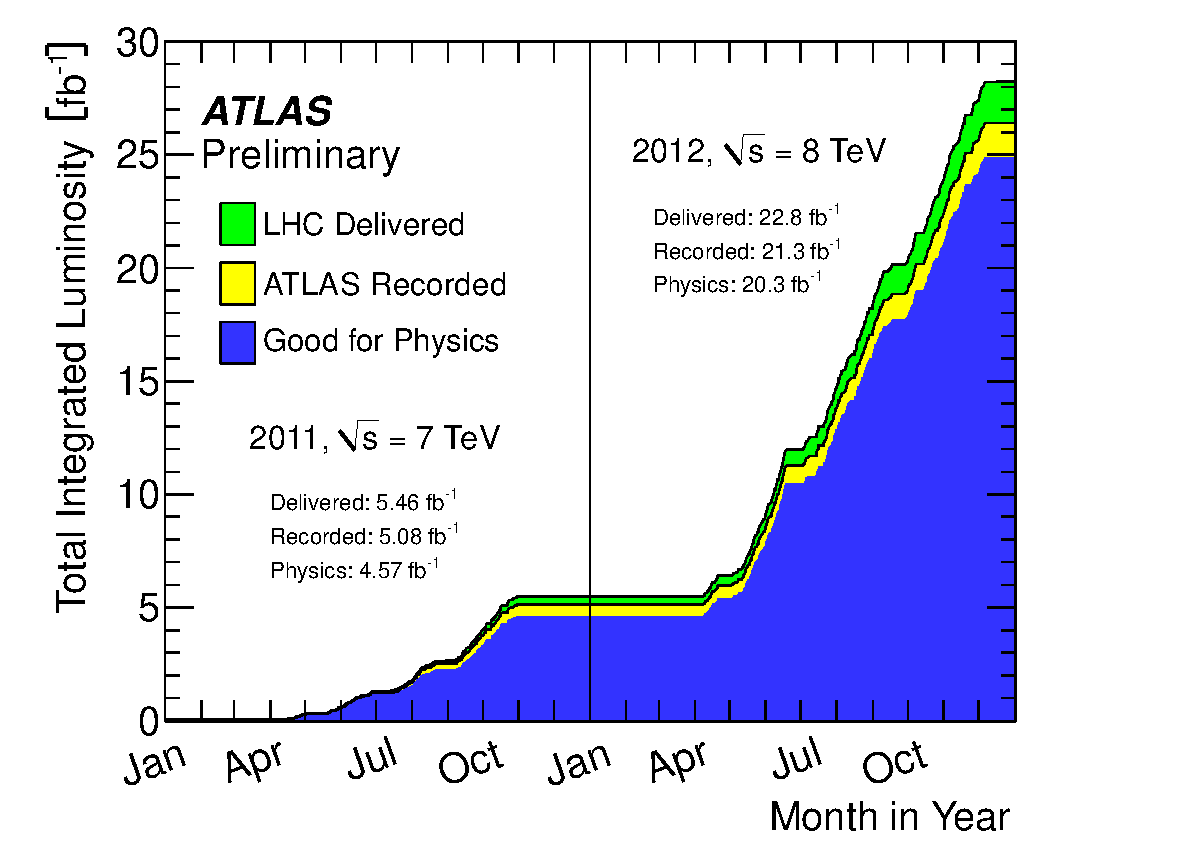
\includegraphics[width=0.60\textwidth]{figs/intlumivstime2011-2012DQ.pdf}
\caption{ Plot showing the accumulation of the integrated lumonisity delivered to the ATLAS experiment over 2011 and 2012. The rough size of the usable, physics ready dataset for 2012 is 20 $fb^-1$ and is the dataset used for the following analysis. 
}
\label{figure:data_lumi}
\end{figure}


\begin{figure}[!t]
\centering 
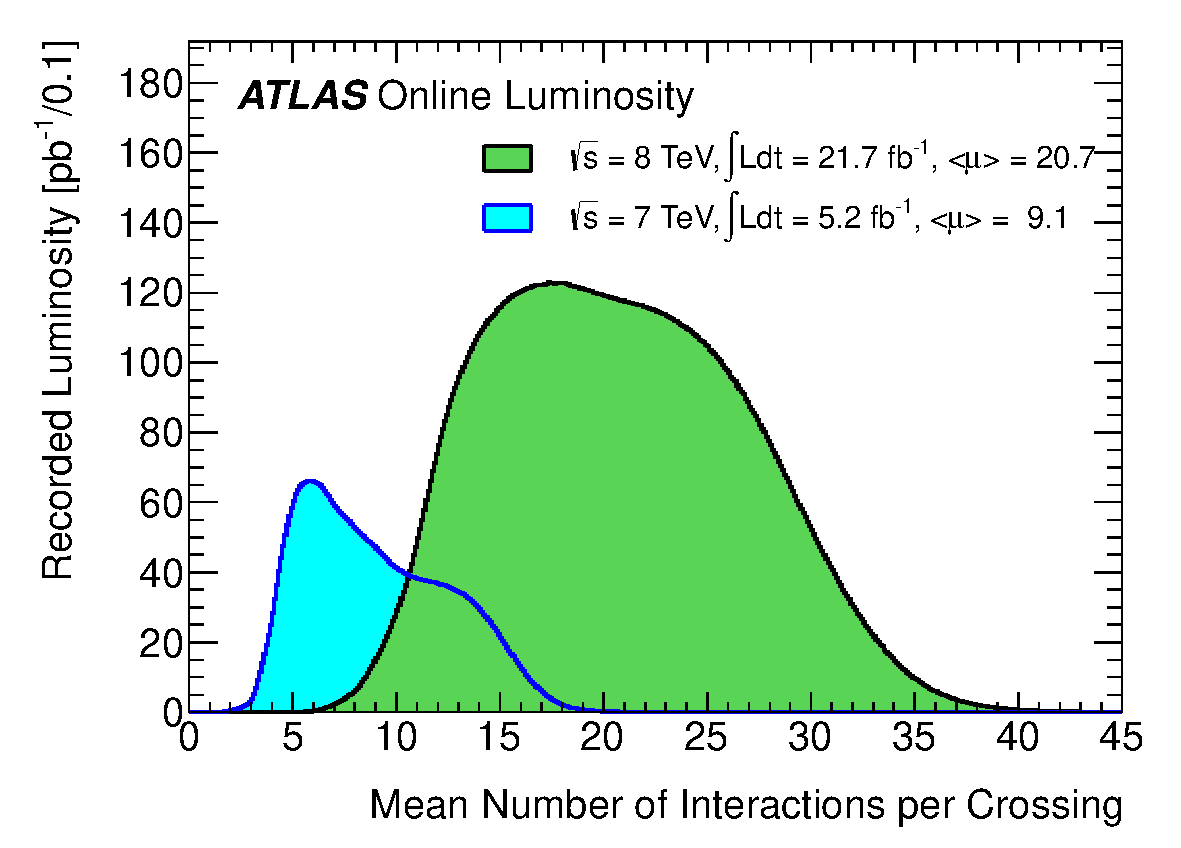
\includegraphics[width=0.60\textwidth]{figs/mu_2011_2012-dec.pdf}
\caption{ The average number of interactions per bunch-crossing for the 2012 and 2011 LHC proton-proton dataset. Most of these interactions are unintersting but leave energetic signatures in particle detectors called pile-up which interfere with measurements}\label{figure:data_pileup}
\end{figure} 

The \tth analysis uses the entire 2012 ATLAS dataset, collected
from April to December. The size of the dataset corresponds to 20.3 \ifb, after passing data quality
requirements, ensuring the proper operation of the tracking, calorimeter and muon subsystems.  

The datasets used in the analysis were collected with the primary electron
(EF\_e24vhi\_medium1 || EF\_e60\_medium1) and muon triggers (
    EF\_24i\_tight || EF\_36\_tight). The electron triggers require a electron
with at least 25 \gev\ of calorimeter energy, passing the medium identification
requirement and loose tracking isolation.  Above 60\gev, the isolation
requirement is dropped and the identification is loosened slightly. Similarly,
            the muon trigger requires a good inner detector track and matching
            hits in the muon spectrometer, as well as loose tracking isolation,
            which also is dropped about 36 \gev\.  The data sample must contain
            either a primary muon or primary electron trigger. 

\section{Simulation}

Simulation samples based on are used to determine the 
overall event selection acceptance and efficiency and for investigations not directly invovled
in the final result The simulated samples are created using parton distribution function (PDF) and
model using Monte Carlo (MC) techniques the hard parton scatter, underlying event activity and parton showering and hadronization. 
The samples are then passed through a full ATLAS detector simulation\cite{Aad:2010ah} based on  GEANT4 \cite{Agostinelli:2002hh}.
Small corrections are then applied to the overall efficiencies to re-scale object identification efficiencies,
      energy scales, and the pile-up, discussed in depth later.  

\subsection{Signal Simulation}


The \ttbar$H$ production is modelled using matrix elements obtained from the HELAC-Oneloop package~\cite{Helac} that corresponds to the next-to-leading order (NLO) QCD accuracy. POWHEG BOX~\cite{powheg,powbox1,powbox2} serves as an interface to the parton shower Monte Carlo programs. The samples created using this approach are referred to as {\textsc PowHel} samples. {\textsc CT10NLO} PDF sets are used and the factorisation ($\mu_{\rm F}$) and renormalization ($\mu_{\rm R}$) scales are set to $\mu_{0} = \mu_{\rm F} = \mu_{\rm R} = m_{t}+\mH/2$. Pile-up and the underlying events are simulated by {\textsc Pythia} 8.1~\cite{PythiaManual8} with the {\textsc CTEQ61L} set of parton distribution functions and AU2 underlying event tune. The Higgs boson mass is set to $125\gev$ and the Top quark mass is set to $172.5\gev$.\\
The signal Monte Carlo samples are summarized in Table~\ref{table:data_mcsignal}.
These large samples are generated with inclusive Higgs boson decays, with
branching fractions set to the LHC Higgs Cross Section Working Group (Yellow Report)
recommendation for $m_H = 125$ GeV \cite{Heinemeyer:2013tqa}.  The inclusive cross section (129.3
fb at $m_H = 125$ GeV) is also obtained from the Yellow Report \cite{Heinemeyer:2013tqa}.



\begin{table}
\begin{center} 
    \caption{Monte Carlo samples used for signal description.}\label{table:data_mcsignal}
   \begin{tabular}{l|c|c|c|c} 

      \hline\hline
       Process & Generator & Cross- & $\mathcal{L}$ [\ifb]  & Detector \\ 
               &           & section [fb] &            &  simulation \\
\hline
 ttH$\rightarrow$allhad+H & PowHel+Pythia8 & 59.09 & 2146.5 & Full \\
 ttH$\rightarrow$ljets+H & PowHel+Pythia8 & 56.63 & 2238.9 & Full \\
 ttH$\rightarrow$ll+H & PowHel+Pythia8 & 13.58 & 9332.0 & Full \\
\hline\hline
    \end{tabular}
  \end{center}
\end{table}


\subsection{Background Simulation}

The background simulations used for this analysis are listed in
Table~\ref{table:data_MCbackground}.  In general, the Alpgen\cite{Mangano:2002ea}, MadGraph\cite{Maltoni:2002qb}, and AcerMC\cite{Kersevan:2004yg} samples use the CTEQ6L1\cite{Nadolsky:2008zw}
parton distribution function, while the Powheg\cite{Frixione:2007vw}, Sherpa\cite{Gleisberg:2008ta}, are generated with the CT10 PDF.  The exception is the MadGraph $t\bar t t \bar t$ sample, which is generated with the
MSTW2008 PDF\cite{Martin:2009iq}. The highest order calculations available are used for cross
sections.  


\begin{table}
\begin{center} 
    \caption{Monte Carlo samples used for background
      description.  Unless otherwise specified MadGraph samples use Pythia 6
      for showering and Alpgen samples use Herwig+Jimmy.}\label{table:data_MCbackground}

\begin{tabular}{l|l|c}
      \hline\hline
       Process & Generator   & Detector \\ 
               &             &  simulation \\
      \hline\hline
\ttW,\ttZ & MadGraph & Full \\
\tZ       & MadGraph & AF2 \\
$t\bar t t \bar t$ & MadGraph & Full \\
\ttWW & Madgraph+Pythia8  & AF2 \\
\ttbar & Powheg+Pythia6  & Full/AF2 \\
single top tchan & AcerMC+Pythia6& Full \\
single top schan$\rightarrow$l   & Powheg+Pythia6 & Full \\
single top $W^{\pm}t$ & Powheg+Pythia6 & Full \\
W$\gamma$*& MadGraph & Full \\
W$\gamma$+4p & Alpgen & Full \\
\WW & Sherpa &  Full \\
\WZ & Sherpa &  Full \\
Same-sign WW & Madgraph+Pythia8 & AF2 \\
ZZ$\rightarrow$ & Powheg+Pythia8,gg2ZZ+Herwig & Full \\
Z$\gamma$*  & Sherpa  & Full \\
Z+jets & Sherpa & Full \\
ggF\_H(125) & Powheg+Pythia8 & Full \\
\end{tabular}
\end{center}
\end{table}



%% \chapter[htoc-titlei][hhead-titlei]{htitlei}
%% -----------------------------------------------------------------------------
\chapter[Conclusions][Conclusions]{Conclusions}

This thesis has presented a preliminary search for the \tth\ process in multilepton
final states using the 2012 8 TeV dataset, collected by ATLAS. The signal regions,
which are binned in number of leptons, show an interesting excess of events. The level of excess is not large enough
to claim statistically signficant observation of a new process, whether SM \tth\ production or otherwise. As
a result, we proceed by setting a 95\% confidence limit on the \tth\ production rate
compared to the SM production,which is much less strict than expected and provide a fitted value of $\mu$,
the ratio of the observed production rate to the theoretical SM \tth\ production rate.

We believe the background processes are well-measured via simple and 
straightforward procedures. These procedures either rely on or are verified by
data control and validation regions surrounding the signal regions. The good
data-MC agreement in these regions suggests that the data excesses are characteristic
of the signal regions only and that the background processes are well-understood
within the systematic uncertainties assigned. 

The signal regions are constructed with simple selection criteria, requiring 
only certain number of leptons, jets, and b-tagged jets within standard
acceptance criteria. Additional selection criteria, namely vetoes of
dilepton invariant mass ranges, are well motivated by the removal
of backgrounds involving Z resonance production. The selection criteria
and background measurement procedures were set prior to viewing the 
data in the signal region.

This analysis shares parts of signal regions with other ATLAS super-symmetric
and exotic analyses, which are under internal review. If similar excesses are seen in these analyses,
it will provide some cross-check to the \tth\ analysis, which is done with a
different procedure for assessing fake background contributions.

This multilepton analysis will be combined with the already public $H\rightarrow b\bar{b}$ \cite{Aad:2014lma} and
$H\rightarrow\gamma\gamma$\cite{ATLAS-CONF-2014-011} analysis, which have observed(expected) 95\%
confidence limits on $\mu$ of 4.1(2.6) and 4.9(6.7), respectively. Both have seen small, non-significant excesses 
with fitted $\mu$ values of 1.7 $\pm$ 1.4 and 1.3 $+$ 2.62 $-$ 1.75, respectively. When approved,
the multilepton analysis will be combined with other analyses in fit constraining the parameters of the Higgs sector.
As it is primarily dependent on the top Yukawa coupling and Higgs coupling to W bosons, it will
have the greatest effect on the measurement of these parameters.

It is interesting to note that the CMS experiment observes a similar excess in their multilepton search
for \tth production. Their observed(expected) 95\% limit on $\mu$ is 6.6(2.4) and their fitted value of $\mu$
is 3.7 $+$ 1.6 $-$ 1.4 \cite{CMS-PAS-HIG-13-020}.

Observing \tth\ production is really a task for the second LHC run. The increased luminosity and collision
energy (13 TeV) will ensure that the \tth\ process is observed with that run's dataset \cite{Dawson:2013bba}. The
overall cross-section of \tth production will increase by a factor of roughly 4, due to accessing
more of the gluon PDFs in the collisions. The cross-sections of most of the backgrounds (\ttV\ and top fakes) will also increase by this factor,
but the increase in the signal cross-section is more important: the second run dataset will have
twice the sensitivity to \tth\ per amount of collected data. While
there will likely not be any conclusive resolution of the excesses found in the multilepton signal regions
with the first run dataset, the second run dataset will surely shed light on this issue.  



%%--------------------------------------------------------------------
%% appendix
%%--------------------------------------------------------------------
%\appendix
%\include{tex/apx-analysis-model}
%\include{tex/apx-tau-vars}
\end{Spacing}

%%--------------------------------------------------------------------
%% bibliography
%%--------------------------------------------------------------------
\backmatter
\bibliographystyle{style/atlasnote}
\bibliography{bibs/theory,bibs/lhc,bibs/data}
%% Add bib files like this:
%% \bibliography{bibs/theory,bibs/atlas}

%%--------------------------------------------------------------------
\end{fmffile}
\end{document}
